\documentclass[12pt,a4paper]{report}

% ---------- Page geometry: A4, 0.7in margins on all sides ----------
\usepackage[a4paper,left=0.7in,right=0.7in,top=0.7in,bottom=0.7in]{geometry}

% ---------- Fonts: Times New Roman substitute ----------
\usepackage{mathptmx}
\usepackage[T1]{fontenc}

% ---------- Line spacing: 1.15 ----------
\usepackage{setspace}
\setstretch{1.15}

% ---------- Headings ----------
\usepackage{titlesec}
\titleformat{\chapter}[block]
  {\centering\bfseries\fontsize{16}{19}\selectfont}
  {CHAPTER \thechapter}{1em}{}
\titlespacing*{\chapter}{0pt}{0pt}{24pt}

\titleformat{\section}
  {\bfseries\fontsize{14}{17}\selectfont}
  {\thesection}{1em}{}

\titleformat{\subsection}
  {\itshape\fontsize{12}{15}\selectfont}
  {\thesubsection}{1em}{}

% ---------- Page numbering: bottom, right-justified ----------
\usepackage{fancyhdr}
\pagestyle{fancy}
\fancyhf{}
\renewcommand{\headrulewidth}{0pt}
\fancyfoot[R]{\thepage}

\fancypagestyle{plain}{%
  \fancyhf{}
  \renewcommand{\headrulewidth}{0pt}
  \fancyfoot[R]{\thepage}
}

% ---------- Figures / tables / graphics ----------
\usepackage{graphicx}
\usepackage{caption}
\captionsetup[figure]{labelfont=bf,name=Figure,labelsep=colon}
\captionsetup[table]{labelfont=bf,name=Table,labelsep=colon}
% Figure captions below figure (default), table captions above table
\captionsetup[table]{position=above}
\captionsetup[figure]{position=below}

% Number figures/tables by chapter, e.g. 1.1, 2.3 (report class default)

\usepackage{amsmath}
\usepackage{enumitem}
\usepackage{xcolor}
\usepackage[hidelinks]{hyperref}
\usepackage[normalem]{ulem}

\title{Machine Learning-Based Content Opportunity 
Ranking and Recommendation System}
\author{Agrim Jain}
\date{August 2026}

\begin{document}

%======================================================================
% TITLE PAGE
%======================================================================
\begin{titlepage}
\thispagestyle{empty}
\begin{center}

\vspace*{1cm}
{\LARGE\bfseries Machine Learning-Based Content Opportunity Ranking and Recommendation System}\par

\vspace{1.5cm}
{\bfseries A SEMINAR REPORT}\par

\vspace{0.1cm}
{\bfseries Submitted in partial fulfilment of the requirements for the award of the degree}\par
{\bfseries of}\par

\vspace{0.5cm}
{\bfseries BACHELOR OF TECHNOLOGY (B.Tech.)}\par
{\bfseries in}\par

\vspace{0.5cm}
{\bfseries Electrical \& Electronics Engineering}\par

\vspace{1.2cm}
{\bfseries Submitted by}\par

\vspace{0.5cm}
{\bfseries{Agrim Jain}}\par
{\bfseries 23FE10EEE00007}\par
{\bfseries VII Semester}\par

\vspace{1.5cm}

\includegraphics[width=3.7in]{Picture1.png}\par

\vspace{1.2cm}
{\bfseries DEPARTMENT OF ELECTRICAL ENGINEERING}\par
{\bfseries MANIPAL UNIVERSITY JAIPUR}\par
{\bfseries JAIPUR-303007}\par
{\bfseries RAJASTHAN, INDIA}\par

\vspace{0.8cm}
{\bfseries AUGUST 2026}\par

\end{center}
\end{titlepage}

%======================================================================
% CERTIFICATE PAGE
%======================================================================
\newpage
\thispagestyle{empty}
\begin{center}
{\bfseries\Large CERTIFICATE}\par
\vspace{1cm}
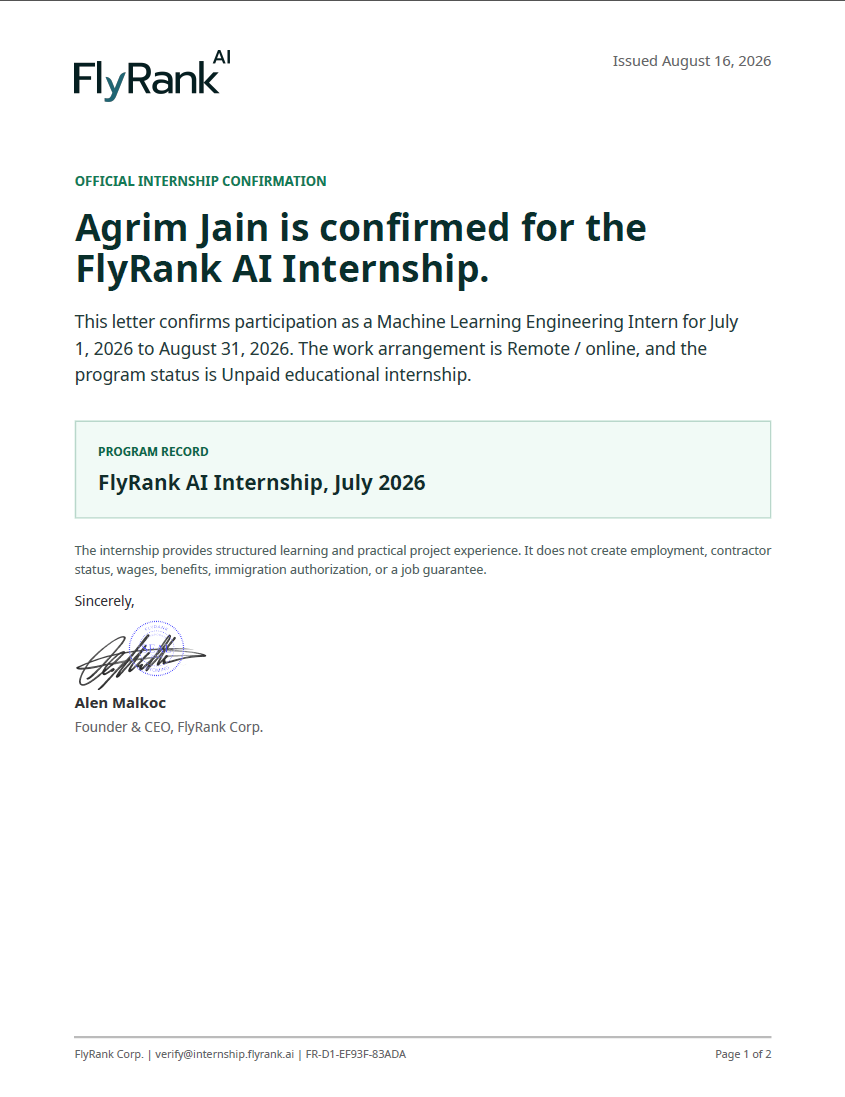
\includegraphics[width=0.95\textwidth]{Screenshot 2026-08-21 191932.png}
\end{center}

%======================================================================
% FRONT MATTER (roman numerals, continuous numbering starts at Ch.1)
%======================================================================
\newpage
\pagenumbering{roman}
\setcounter{page}{1}

\chapter*{ACKNOWLEDGMENTS}
\addcontentsline{toc}{chapter}{ACKNOWLEDGMENTS}

I would like to express my sincere gratitude to everyone who contributed to the successful completion of my project titled ``Machine Learning-Based Content Opportunity Ranking and Recommendation System.'' This project has been a valuable learning experience, allowing me to apply my knowledge of Machine Learning and Artificial Intelligence to a practical problem involving data analysis, model development, evaluation, ranking, and recommendation generation.

I am grateful to the Dean/Associate Dean of Manipal University Jaipur for providing an academic environment that encourages innovation and project-based learning. I sincerely thank the Head of the Department of Electrical and Electronics Engineering, Dr. Neeraj Kanwar Ma'am, for her guidance, encouragement, and support throughout my academic journey.

I extend my special gratitude to my Project Supervisor and Mentor, Mirza Asceric, for his valuable guidance, feedback, and continuous support throughout the project. His mentorship helped me develop a structured understanding of problem formulation, data safety, feature selection, baseline development, model evaluation, ranking metrics, and result interpretation.

I am also thankful to FlyRank AI for providing me with the opportunity to work on this capstone project and gain practical exposure to a real-world machine learning workflow. The project helped me understand the practical application of machine learning through data analysis, model comparison, ranking evaluation, feature importance analysis, and recommendation generation.

I would also like to thank the Department Project Coordinator, Co-coordinator, Department Guide, Laboratory In-charge, and all faculty members of the Department of Electrical and Electronics Engineering for their guidance and support throughout my studies and project work.

Finally, I express my heartfelt gratitude to my parents, family, friends, and classmates for their constant encouragement and support. The knowledge and practical experience gained through this project have strengthened my interest in Machine Learning and Artificial Intelligence and will provide a valuable foundation for my future academic and professional endeavours.

\vspace{1cm}
\textbf{Agrim Jain}\par
\textbf{23FE10EEE00007}

\chapter*{ABSTRACT}
\addcontentsline{toc}{chapter}{ABSTRACT}
The rapid growth of digital content and search-driven platforms has made it increasingly difficult to manually identify and prioritize content items for review. Large content collections vary in search demand, ranking position, content characteristics, and other performance-related signals, making manual prioritization inefficient and subjective. This project develops a Machine Learning-Based Content Opportunity Ranking and Recommendation System that prioritizes content records according to their potential opportunity for human review. The system is designed as a transparent and reproducible decision-support tool rather than an attempt to predict proprietary search engine algorithms or automatically prescribe content changes.

The project uses the Ranking Lifecycle dataset provided through the FlyRank AI ML Internship dataset, consisting of 205,749 observations, 34 variables, and 54 pseudonymized clients. The methodology includes exploratory data analysis, missing-value analysis, feature selection, leakage-aware preprocessing, opportunity score construction, and development of a transparent baseline. Client-aware splitting was used to divide the data into training, validation, and test sets. ElasticNet, Random Forest, Histogram-Based Gradient Boosting, XGBoost, and LightGBM were evaluated using Spearman correlation, Precision@K, and Normalized Discounted Cumulative Gain (NDCG@K). Histogram-Based Gradient Boosting was selected as the final model based on validation performance, followed by feature importance analysis.

The results show that machine learning can capture useful relationships among content and search-related signals for opportunity ranking. Content age was identified as the strongest contributing feature, while search intent and selected structural features provided additional information. The final model achieved competitive ranking performance and outperformed the Age Baseline on selected measures, including Spearman correlation and certain NDCG cutoffs. However, the baseline remained competitive and performed better on some evaluation points, highlighting the importance of comparing complex models with simple and interpretable alternatives. Differences between training and test distributions further emphasized the need for careful evaluation and interpretation.

Overall, the project demonstrates the potential of machine learning as a decision-support tool for prioritizing content records for human review. The system generates opportunity scores and ranked recommendations to reduce the effort required to examine large collections of records. The findings also demonstrate that a more complex model does not necessarily outperform a simple baseline across all metrics. Future work can focus on improving the opportunity target, incorporating additional temporal and content-level features, evaluating performance across broader client and time ranges, and incorporating human feedback into the recommendation process.


\listoftables
\addcontentsline{toc}{chapter}{LIST OF TABLES}

\listoffigures
\addcontentsline{toc}{chapter}{LIST OF FIGURES}

\tableofcontents

%======================================================================
% MAIN MATTER (arabic numerals, continuous numbering from Chapter 1)
%======================================================================
\newpage
\pagenumbering{arabic}
\setcounter{page}{1}

%----------------------------------------------------------------------
\chapter{INTRODUCTION}

\section{\textit{Background}}
The rapid growth of digital content and online information has created challenges for organizations in managing and prioritizing large volumes of content. Websites may contain hundreds or thousands of pages targeting different search queries, user intents, and levels of search demand. Manually evaluating each content item to determine which pages require attention can be time-consuming and inefficient. Therefore, systematic approaches are needed to analyse available signals and identify records that may require earlier review.

Search-related data provides several useful signals for evaluating digital content, including search volume, impressions, clicks, click-through rate, average ranking position, content age, content type, search intent, and structural characteristics. Analysing these variables independently, however, may not provide a complete view of potential content opportunities. For example, a page with high search demand and a strong ranking position may require less immediate attention than one with meaningful demand but a relatively weaker position. This creates a need to combine multiple signals for effective prioritization.

Machine learning can support this process by learning relationships among multiple input variables and generating scores that can be used to rank observations according to a defined objective. Such systems can process large datasets efficiently and provide a consistent approach to prioritization. However, their effectiveness depends on appropriate feature selection, prevention of data leakage, model evaluation, interpretability, and comparison with simple baseline methods.

This project develops a \textbf{Machine Learning-Based Content Opportunity Ranking and Recommendation System} using the Ranking Lifecycle dataset provided through the FlyRank AI ML Internship program. The dataset contains \textbf{205,749 observations}, \textbf{34 variables}, and records associated with \textbf{54 pseudonymized clients}. The data includes content-related, search-related, structural, and engagement-related variables. The project investigates how selected features can be used to construct an opportunity-oriented ranking system for prioritizing content records for human review. The proposed system is designed to support decision-making rather than automatically modify content. It generates opportunity scores and ranked outputs to identify records that may warrant further investigation. An Age-Based Baseline is used as a transparent reference for evaluating machine learning models. Multiple models are assessed using ranking-oriented metrics, including Spearman rank correlation, Precision@K, and Normalized Discounted Cumulative Gain (NDCG@K).

Overall, the project demonstrates a structured machine learning workflow covering data exploration, leakage-aware feature selection, baseline construction, model training, validation, evaluation, interpretation, and recommendation generation. The objective is to provide a transparent and reproducible approach for prioritizing content opportunities while recognizing the limitations of automated ranking systems.


\section{\textit{Problem Statement}}
The increasing volume of digital content creates a practical challenge in determining which content records should receive attention first. Large datasets may contain records with different levels of search demand, ranking positions, content characteristics, and engagement signals. Reviewing all records manually is inefficient, while relying on a single metric may overlook the interaction between multiple factors.

For example, a record with high search volume and a strong ranking position may require less immediate attention than one with meaningful demand but a weaker ranking position. Therefore, identifying content opportunities requires combining multiple signals within a consistent prioritization framework.

The problem addressed in this project is the development of a systematic approach for \textbf{ranking and prioritizing content records according to their potential opportunity for human review}. The system does not automatically determine whether content should be modified or attempt to predict proprietary search engine behaviour. Instead, it generates an opportunity-oriented score to rank records and support human decision-making.

Another challenge is determining whether machine learning provides additional value over a simple and transparent approach. Therefore, multiple machine learning models are compared with a transparent \textbf{Age-Based Baseline} using the same ranking-oriented evaluation framework.

The problem can therefore be summarized as follows:

\begin{quote}
\itshape
\uline{How can available content, search, and structural signals be used to develop a transparent and reproducible system that ranks content records according to their potential opportunity for human review, while evaluating whether machine learning provides additional value over a simple baseline?}
\end{quote}

To address this problem, the project evaluates multiple machine learning models using selected features and ranking-oriented metrics. The resulting system produces opportunity scores and ranked outputs that can assist human reviewers in identifying records that may require earlier investigation.

\section{\textit{Need for the Project}}
The increasing scale of digital content makes effective prioritization an important practical requirement. Organizations may manage large collections of records with different search demand, ranking positions, content age, search intent, and structural characteristics. Analysing these records individually can be time-consuming, creating a need for a systematic approach to identify which records should be examined first.

Simple prioritization based on a single metric may not provide a complete view of content opportunity. For example, high search volume may identify pages that already perform well, while weak ranking positions may include records with limited demand. A useful system should therefore combine multiple signals and produce a ranked output based on a defined objective.

The project also addresses the need for \textbf{decision support} in data-driven workflows. A ranking system can reduce the number of records requiring detailed manual review and help direct human effort toward potentially relevant candidates. The system is intended to support, rather than replace, human judgment, as the available data may not capture every factor required for a final content-related decision.

Another requirement is to evaluate machine learning against a transparent baseline. Although machine learning can capture relationships among multiple variables, its additional complexity should be supported by measurable performance improvements. A simple baseline therefore provides an important reference for assessing the practical value of the proposed models.

The project establishes a \textbf{transparent, reproducible, and data-driven framework} for content opportunity prioritization through exploratory analysis, leakage-aware feature selection, baseline development, machine learning evaluation, and ranking-oriented metrics. The need for this work can be summarized as follows:

\begin{itemize}[leftmargin=*]
\item To reduce the manual effort required to review large numbers of content records.
\item To combine multiple content, search, and structural signals rather than relying on a single metric.
\item To rank records according to a defined opportunity objective.
\item To evaluate machine learning against a transparent baseline.
\item To provide interpretable outputs that support human decision-making.
\item To establish a reproducible workflow covering data safety, feature selection, model evaluation, and result interpretation.
\end{itemize}

\section{\textit{Aim of the Project}}

The aim of this project is to develop a \textbf{Machine Learning-Based Content Opportunity Ranking and Recommendation System} that uses available content, search, and structural signals to prioritize content records according to their potential opportunity for human review. The proposed system is designed as a \textbf{decision-support framework} rather than an automated content modification system. Its purpose is to analyse many content records, generate an opportunity-oriented score, and produce a ranked output that helps human reviewers identify records that may deserve earlier investigation. To achieve this aim, the project incorporates exploratory data analysis, leakage-aware feature selection, opportunity score construction, baseline development, machine learning model training, validation, ranking-oriented evaluation, and model interpretation. A transparent \textbf{Age-Based Baseline} is used as a reference for evaluating whether the selected machine learning approach provides additional value. The final objective is to establish a \textbf{transparent, reproducible, and interpretable workflow} that demonstrates how machine learning can be applied to prioritize content records while clearly communicating the performance, limitations, and appropriate use of the generated recommendations.

\section{\textit{Objectives of the Project}}
The main objective of this project is to develop a machine learning-based system for ranking and prioritizing content records according to their potential opportunity for human review. The specific objectives are:

\begin{enumerate}[leftmargin=*]
\item To analyse the dataset and understand the characteristics, distributions, missing values, and relationships among content, search, structural, and engagement-related variables.
\item To identify suitable features for the ranking task while considering data safety, pseudonymous identifiers, missing values, and potential data leakage.
\item To construct an opportunity-oriented scoring framework for prioritizing content records.
\item To develop a transparent Age-Based Baseline for comparison with machine learning approaches.
\item To divide the dataset into training, validation, and test sets using a structured splitting strategy.
\item To develop and compare ElasticNet, Random Forest, Histogram-Based Gradient Boosting, XGBoost, and LightGBM models.
\item To evaluate model performance using Spearman rank correlation, Precision@K, and NDCG@K.
\item To compare the selected machine learning model with the Age-Based Baseline and assess its additional value.
\item To analyse feature importance and interpret the factors contributing to the generated opportunity scores.
\item To generate ranked recommendations and reason codes to assist human reviewers in identifying records for further investigation.
\item To establish a transparent and reproducible workflow covering data analysis, preprocessing, model development, evaluation, interpretation, and recommendation generation.
\end{enumerate}

\section{\textit{Scope of the Project}}
The scope of this project focuses on developing and evaluating a \textbf{Machine Learning-Based Content Opportunity Ranking and Recommendation System} using structured data from the FlyRank AI ML Internship dataset. The project covers the workflow required to transform the available data into a ranking-oriented decision-support system. The work includes exploratory data analysis, missing-value analysis, feature selection, preprocessing, and consideration of data leakage. Pseudonymous identifier columns are excluded from the machine learning feature set. An opportunity-oriented scoring framework and a transparent \textbf{Age-Based Baseline} are developed for comparison with multiple machine learning models, including ElasticNet Regression, Random Forest, Histogram-Based Gradient Boosting, XGBoost, and LightGBM.

The models are evaluated using separate training, validation, and test datasets. Since the primary objective is ranking, performance is assessed using Spearman rank correlation, Precision@K, and Normalized Discounted Cumulative Gain at K (NDCG@K). The project also includes feature importance analysis and comparison of the selected machine learning model with the baseline. The final system generates opportunity scores, ranked content records, and supporting reason codes to assist human reviewers in identifying records that may require earlier investigation. However, the project does not attempt to predict proprietary search engine algorithms, guarantee improvements in search rankings, or automatically modify website content. The generated scores and recommendations are intended as a \textbf{decision-support mechanism}, with final decisions remaining dependent on human judgment and additional contextual information.

%----------------------------------------------------------------------
\chapter{BACKGROUND THEORY}

\section{\textit{Introduction to Content Opportunity Analysis}}
Digital platforms often contain large numbers of content pages covering different topics, search queries, and audiences. As content volume increases, differences in search demand, ranking position, content characteristics, age, and engagement make manual review increasingly difficult. A systematic approach is therefore needed to identify records that may deserve further investigation. Content opportunity analysis involves examining multiple signals associated with content records to identify potentially relevant opportunities for human review. No single variable may provide sufficient information for prioritization. For example, a record with high search demand may already have a strong ranking position, while a record with a weaker position may have limited demand. Combining multiple signals can therefore provide a more structured basis for prioritization.

Relevant signals may include search volume, average search position, content age, content type, search intent, keyword characteristics, title characteristics, and URL structure. These variables can be combined to assign an opportunity score and produce a ranked list of records. Such a ranking reduces the number of records requiring detailed manual examination and allows reviewers to focus on higher-priority candidates. Since the objective is to prioritize relevant records near the top of the ranking, ranking-oriented metrics such as Spearman rank correlation, Precision@K, and Normalized Discounted Cumulative Gain at K (NDCG@K) are appropriate for evaluating the system.

The resulting scores should not be interpreted as guaranteed predictions of future search performance or proprietary search engine behaviour. They depend on the available data, selected features, opportunity definition, preprocessing, and evaluation methodology. Therefore, the ranking is intended to support human decision-making rather than replace it. In this project, content opportunity analysis forms the foundation of the proposed \textbf{Machine Learning-Based Content Opportunity Ranking and Recommendation System}. Selected content, search, and structural variables are used to generate opportunity-oriented scores and prioritize records for further human review.

\section{\textit{Search Ranking and Content Performance}}

Search ranking and content performance provide measurable signals for understanding how content records perform within the available dataset. Variables such as search volume, impressions, clicks, click-through rate (CTR), average position, and engagement measures describe different aspects of observed performance and can help identify records for further investigation.

\textbf{Search volume} indicates the observed demand associated with a keyword or search topic. However, it should not be considered independently. A high-demand keyword with a strong search position may represent a different opportunity from one with similar demand but a weaker position.

\textbf{Average position} represents the observed ranking position of a content record. A lower numerical value generally indicates a stronger position, while a higher value indicates a weaker position. Its usefulness for prioritization depends on other signals, particularly search demand and content context.

\textbf{Impressions and clicks} provide information about search visibility and user interaction. Their relationship can be represented through the \textbf{Click-Through Rate (CTR)}:

\begin{equation}
CTR = \frac{\text{Clicks}}{\text{Impressions}} \times 100
\label{eq:ctr}
\end{equation}

CTR indicates the proportion of impressions that result in clicks, although user behaviour may be influenced by factors not represented in the dataset.

The dataset also contains engagement-related variables such as pageviews, sessions, users, engaged sessions, AI sessions, scroll events, engagement rate, scroll rate, and AI traffic percentage. These variables provide additional information about observed user activity, but differences in data availability and missing values require consideration during preprocessing and feature selection. Overall, search and performance signals should be considered together rather than in isolation. In this project, these signals contribute to the opportunity-oriented ranking framework, where selected features are used to prioritize records for human review. The resulting rankings are not intended to guarantee future performance improvements or predict proprietary search engine behaviour.

\section{\textit{Machine Learning for Content Prioritization}}
Machine learning provides a systematic approach for analysing large datasets containing multiple variables and identifying patterns that may not be evident through manual analysis. In content prioritization, records may differ in search demand, ranking position, content properties, search intent, and structural characteristics. A machine learning model can learn relationships among selected features and generate scores that can be used to rank records. The machine learning workflow begins with data preparation, including understanding variables, analysing missing values and duplicates, examining distributions, and selecting appropriate features. Pseudonymous identifiers may be useful for grouping or data splitting but should not be used as predictive features. Similarly, potential leakage must be addressed to ensure meaningful model evaluation.

After preprocessing, the model is trained using selected features and a defined target or reference score. It then generates scores for unseen observations, which can be ordered according to the defined opportunity objective. Thus, the purpose of machine learning in this project is not only prediction but also prioritization of records for human review. Different algorithms capture different types of relationships. Linear models provide simpler relationships, while tree-based ensemble methods can capture nonlinear patterns and feature interactions. Therefore, the project evaluates ElasticNet Regression, Random Forest, Histogram-Based Gradient Boosting, XGBoost, and LightGBM.

A key advantage of machine learning is its ability to combine multiple variables into a single scoring mechanism. However, greater complexity does not necessarily guarantee better performance. The models must therefore be compared with a transparent baseline using the same data splits and evaluation framework. Since the primary objective is ranking, ranking-oriented metrics are more appropriate than prediction metrics alone. Spearman rank correlation, Precision@K, and NDCG@K are used to evaluate whether high-priority records are placed near the top of the generated ranking.

Machine learning outputs must also be interpreted carefully. A high opportunity score is not a guaranteed outcome or causal conclusion; it reflects patterns learned from the selected features and the defined opportunity objective. The resulting ranking is therefore treated as a decision-support output rather than a replacement for human judgment. Overall, machine learning forms part of a broader framework involving data exploration, feature selection, baseline development, model comparison, ranking evaluation, interpretation, and recommendation generation. This enables the usefulness of machine learning to be assessed transparently against a simpler alternative.

\section{\textit{Supervised Machine Learning}}
Supervised machine learning is a branch of machine learning in which a model learns the relationship between input features and a known target or reference output. The general relationship can be represented as:

\begin{equation}
\hat{y} = f(X)
\end{equation}

where $X$ represents the input features, $f$ represents the learned model, and $\hat{y}$ represents the predicted output.

In this project, selected content, search, and structural features are used to generate an opportunity-oriented score for each content record. These scores are then used to rank records according to the defined opportunity objective.

The supervised learning process consists of training, validation, and testing. Candidate models are trained on the training dataset, compared on the validation dataset, and the selected model is finally evaluated on the separate test dataset. This separation helps assess how well the model generalizes to previously unseen data.

The dataset used for supervised learning can be represented as:

\begin{equation}
D = \{(X_i, y_i)\}_{i=1}^{n}
\end{equation}

where $X_i$ represents the feature vector of the $i^{th}$ observation and $y_i$ represents its corresponding target or reference value.

The workflow followed in this project is:

\begin{enumerate}[leftmargin=*]
    \item \textbf{Feature Selection:} Relevant features are selected while excluding pseudonymous identifiers and potential sources of data leakage.
    \item \textbf{Data Splitting:} The dataset is divided into training, validation, and test sets.
    \item \textbf{Model Training:} Candidate models are trained using the selected features and training data.
    \item \textbf{Validation:} Candidate models are compared using the validation dataset and selected evaluation metrics.
    \item \textbf{Final Evaluation:} The selected model is evaluated on the separate test dataset.
\end{enumerate}

Unlike a traditional classification problem, the present project uses supervised learning primarily as a scoring and ranking mechanism. The model generates a continuous opportunity score, which is used to order records from higher to lower priority. Therefore, model performance is assessed based on both the generated scores and the quality of the resulting rankings.

The project evaluates five supervised machine learning models: \textbf{ElasticNet Regression}, \textbf{Random Forest}, \textbf{Histogram-Based Gradient Boosting}, \textbf{XGBoost}, and \textbf{LightGBM}. Their comparative evaluation helps determine the effectiveness of different modelling approaches for the defined ranking objective.

\section{\textit{Baseline Models}}
A baseline model provides a simple and transparent reference for evaluating more complex machine learning models. Its purpose is not necessarily to achieve the highest performance, but to determine whether a more complex approach provides meaningful additional value. Baselines are particularly useful in ranking problems because simple rules can provide an interpretable and reproducible initial ranking. Comparing such a ranking with machine learning models helps determine whether the additional model complexity is justified. In this project, an \textbf{Age-Based Baseline} was developed using the \texttt{content\_age\_days} variable. This variable was selected because exploratory analysis showed the strongest observed Spearman correlation with the constructed opportunity score among the available non-leakage candidate features.

The baseline can be conceptually represented as:

\begin{equation}
\text{Baseline Score} = g(\text{Content Age})
\end{equation}

where $g$ represents the rule or transformation used to convert content age into a baseline score. The resulting scores are used to rank the content records.

The baseline is intentionally simple and does not capture interactions among multiple features. It instead provides a transparent reference for determining whether machine learning can provide additional ranking information. For a fair comparison, the baseline and machine learning models are evaluated using the same data splits and ranking metrics, including \textbf{Spearman rank correlation}, \textbf{Precision@K}, and \textbf{NDCG@K}.

Thus, the Age-Based Baseline provides an important reference for interpreting model performance. If a machine learning model performs better, the improvement may indicate that the selected features provide additional ranking information beyond content age alone. Conversely, competitive baseline performance highlights the value of considering simpler alternatives.

\subsection{\textit{Machine Learning Models}}

Multiple machine learning models were evaluated to compare different approaches for learning the relationship between the selected input features and the constructed opportunity-oriented target. Using multiple models allows the project to compare algorithms with different levels of complexity and modelling capabilities rather than assuming that a particular approach will perform best. The evaluated models include \textbf{ElasticNet Regression}, \textbf{Random Forest}, \textbf{Histogram-Based Gradient Boosting}, \textbf{XGBoost}, and \textbf{LightGBM}. These models provide a comparison between a regularized linear approach and tree-based ensemble methods capable of modelling nonlinear relationships and feature interactions. \textbf{ElasticNet Regression} provides a relatively simple and regularized linear approach, while \textbf{Random Forest}, \textbf{Histogram-Based Gradient Boosting}, \textbf{XGBoost}, and \textbf{LightGBM} use tree-based methods to capture more complex relationships within the data. Comparing these approaches helps determine whether increased model complexity provides meaningful improvements for the defined ranking objective. All candidate models are trained and evaluated within the same experimental framework. Their performance is compared using the validation dataset and ranking-oriented metrics, including \textbf{Spearman Rank Correlation}, \textbf{Precision@K}, and \textbf{Normalized Discounted Cumulative Gain at K (NDCG@K)}.

The following subsections provide a brief theoretical overview of each machine learning model used in the project.

\subsubsection{\textit{ElasticNet Regression}}
ElasticNet Regression is a regularized linear regression technique that combines the properties of Ridge and Lasso Regression. It models the relationship between input features and a continuous target while controlling model complexity through regularization. A general linear regression model can be represented as:

\begin{equation}
\hat{y} = \beta_0 + \beta_1x_1 + \beta_2x_2 + \cdots + \beta_px_p
\end{equation}

where $\hat{y}$ represents the predicted output, $\beta_0$ is the intercept, $\beta_1,\ldots,\beta_p$ are the feature coefficients, and $x_1,\ldots,x_p$ are the corresponding feature values. ElasticNet applies both L1 and L2 regularization. The L1 component encourages sparsity by reducing the influence of less important features, while the L2 component penalizes large coefficient values and improves stability when features are correlated. The objective can be conceptually represented as:

\begin{equation}
\text{Loss} =
\text{Prediction Error}
+
\text{L1 Regularization}
+
\text{L2 Regularization}
\end{equation}

The balance between the two regularization components is controlled through model parameters, allowing ElasticNet to combine the feature-selection behaviour of Lasso with the coefficient stabilization of Ridge Regression. In this project, ElasticNet Regression was used as a relatively simple and interpretable model for generating continuous opportunity-oriented scores from the selected content, search, and structural features. Its inclusion provides a linear reference against which the nonlinear tree-based models can be compared. Since ElasticNet primarily models linear relationships, it may be less effective at automatically capturing complex nonlinear patterns and feature interactions. Its performance was therefore evaluated using the same ranking-oriented framework as the other candidate models, including \textbf{Spearman Rank Correlation}, \textbf{Precision@K}, and \textbf{NDCG@K}.


\subsubsection{\textit{Random Forest}}

Random Forest is an ensemble machine learning algorithm that combines multiple decision trees to produce a final prediction. It reduces the sensitivity and overfitting associated with individual decision trees by introducing randomness during tree construction and aggregating their outputs. The algorithm uses two main sources of randomness. Each tree is trained on a different random sample of the training data, and a random subset of features is considered at each split. This creates diversity among the trees and improves the stability of the overall model.

For a regression problem, the final prediction can be represented as:

\begin{equation}
\hat{y} =
\frac{1}{M}
\sum_{m=1}^{M}
T_m(X)
\end{equation}

where $\hat{y}$ is the final predicted output, $M$ is the number of decision trees, and $T_m(X)$ is the prediction from the $m^{th}$ tree.

Random Forest can capture non linear relationships and feature interactions without requiring them to be explicitly defined. This makes it suitable for structured datasets where the relationship between features and the target may be complex. It can also model both linear and non linear patterns without strong assumptions about the underlying data distribution. In this project, the \textbf{Random Forest Regressor} was used to generate continuous opportunity-oriented scores from the selected content, search, and structural features. The predicted scores were subsequently used to rank content records. Although Random Forest provides flexibility and robustness, its predictions are less directly interpretable than those of a simple linear model and may require greater computational resources when using many trees. Its performance was evaluated using the same ranking-oriented framework as the other candidate models, including \textbf{Spearman Rank Correlation}, \textbf{Precision@K}, and \textbf{NDCG@K}. The inclusion of Random Forest provides a non linear ensemble approach for comparison with ElasticNet Regression and the gradient boosting models used in the project.

\subsubsection{\textit{Histogram-Based Gradient Boosting}}

Histogram-Based Gradient Boosting is an ensemble learning technique based on gradient boosting, where decision trees are added sequentially to reduce the errors of the existing model. The overall prediction can be represented as:

\begin{equation}
F_M(X) = \sum_{m=1}^{M} \gamma_m h_m(X)
\end{equation}

where $F_M(X)$ is the final prediction after $M$ boosting stages, $h_m(X)$ is the prediction from the $m^{th}$ decision tree, and $\gamma_m$ represents its contribution.

In gradient boosting, each successive tree is trained to improve the predictions of the previous model. This sequential process enables the model to capture complex relationships between input features and the target. Histogram-Based Gradient Boosting improves computational efficiency by grouping continuous feature values into discrete bins. Instead of evaluating every possible split point, the algorithm evaluates splits using these histogram bins, reducing computational cost for large datasets. In this project, the \textbf{HistGradientBoosting Regressor} was used to generate continuous opportunity-oriented scores from the selected content, search, and structural features. Its tree-based structure allows it to capture nonlinear relationships and feature interactions without requiring them to be explicitly specified.

The histogram-based approach is particularly suitable for the project's large structured dataset because it provides efficient training while retaining the flexibility of tree-based models. However, its effectiveness was determined through experimental evaluation rather than assumed from its complexity. The model was evaluated using \textbf{Spearman Rank Correlation}, \textbf{Precision@K}, and \textbf{NDCG@K}, and was compared with the other candidate models and the transparent Age-Based Baseline. Based on validation performance, Histogram-Based Gradient Boosting was selected as the final machine learning model for the project. The selected model generates opportunity-oriented scores that are used to rank content records and support human review.

\subsubsection{\textit{XGBoost}}

XGBoost (Extreme Gradient Boosting) is a gradient boosting algorithm designed for efficient learning on structured data. It builds an ensemble of decision trees sequentially, with each new tree improving the predictions of the existing ensemble. The final prediction can be represented as:

\begin{equation}
\hat{y} =
\sum_{m=1}^{M}
f_m(X)
\end{equation}

where $\hat{y}$ is the predicted output, $M$ is the number of trees, and $f_m(X)$ represents the contribution of the $m^{th}$ tree.

XGBoost uses gradient-based optimization to reduce prediction errors during successive boosting stages. It also incorporates regularization to control model complexity and reduce the risk of overfitting. Its tree-based structure enables the model to capture nonlinear relationships and interactions between input features. In this project, the \textbf{XGBoost Regressor} was used to generate continuous opportunity-oriented scores from the selected content, search, and structural features. These predicted scores were subsequently used to rank content records according to the defined opportunity objective.

Model performance can be influenced by parameters such as the number of trees, learning rate, and tree depth. These parameters affect model complexity and generalization. Therefore, XGBoost was evaluated within the same experimental framework as the other candidate models rather than assuming that its greater flexibility would result in better performance. The model was evaluated using \textbf{Spearman Rank Correlation}, \textbf{Precision@K}, and \textbf{NDCG@K}, and its performance was compared with the Age-Based Baseline and other candidate models. Its inclusion provided an additional gradient boosting approach for assessing whether greater modelling flexibility could improve the content opportunity ranking task.


\subsubsection{\textit{LightGBM}}
LightGBM (Light Gradient Boosting Machine) is a gradient boosting framework designed for efficient learning on large structured datasets. It builds decision trees sequentially, with each tree improving the predictions of the existing ensemble. The final prediction can be represented as:

\begin{equation}
\hat{y} =
\sum_{m=1}^{M}
f_m(X)
\end{equation}

where $\hat{y}$ is the final predicted output, $M$ is the number of decision trees, and $f_m(X)$ represents the contribution of the $m^{th}$ tree.

LightGBM uses a histogram-based approach that groups continuous feature values into discrete bins, reducing the computational effort and memory requirements during tree construction. It can also capture nonlinear relationships and interactions between input features without requiring them to be explicitly defined.

Another characteristic of LightGBM is its leaf-wise tree growth strategy, which expands the leaf providing the greatest reduction in the objective function. This can improve learning efficiency but requires appropriate parameter selection to control model complexity and overfitting.

In this project, the \textbf{LightGBM Regressor} was used as a candidate model for generating continuous opportunity-oriented scores from the selected content, search, and structural features. The resulting scores were used to rank content records according to the defined opportunity objective.

LightGBM performance is influenced by parameters such as the number of estimators, learning rate, number of leaves, tree depth, feature sampling, and regularization. Therefore, its effectiveness was determined through experimental evaluation rather than assumed from its computational efficiency or model complexity.

The model was evaluated using \textbf{Spearman Rank Correlation}, \textbf{Precision@K}, and \textbf{NDCG@K} within the same validation framework as the other candidate models. Its results were compared with the Age-Based Baseline, ElasticNet Regression, Random Forest, Histogram-Based Gradient Boosting, and XGBoost.

The inclusion of LightGBM provides an efficient gradient boosting approach for the content opportunity ranking task, with the final model selection based on measured validation and test performance.

\section{\textit{Ranking Evaluation Metrics}}

Since the primary objective of the proposed system is to rank content records according to their predicted opportunity scores, model evaluation focuses on ranking performance rather than conventional regression measures. A model may produce reasonable numerical predictions while still failing to place high-priority records near the top of the ranking. Ranking metrics measure different aspects of ranking quality. Some assess agreement between predicted and reference rankings, while others focus on the relevance of the highest-ranked records. This distinction is important because top-ranked records are likely to receive greater attention during human review.

The project uses three primary ranking metrics:

\begin{enumerate}[leftmargin=*]
    \item \textbf{Spearman Rank Correlation:} Measures the agreement between predicted and reference rankings.
    \item \textbf{Precision@K:} Measures the proportion of relevant records among the top $K$ ranked observations.
    \item \textbf{Normalized Discounted Cumulative Gain (NDCG@K):} Evaluates ranking quality while giving greater importance to relevant records appearing at higher positions.
\end{enumerate}

These metrics provide complementary views of performance. Spearman Rank Correlation evaluates overall ranking consistency, while Precision@K and NDCG@K focus more directly on the quality and relevance of the top-ranked records. Using multiple metrics is important because a model may perform well on overall rank agreement but less effectively at identifying the most relevant records near the top. Similarly, performance may vary across different values of $K$. Therefore, the Age-Based Baseline and candidate machine learning models are evaluated using the same dataset splits and ranking-oriented metrics to ensure consistent comparison. The following subsections describe each metric used in the project.

\subsection{\textit{Spearman Rank Correlation}}

Spearman Rank Correlation is a non-parametric measure used to evaluate the strength and direction of the relationship between two ranked variables. Unlike Pearson correlation, it evaluates the consistency of the ordering between variables rather than their direct numerical relationship. In a ranking problem, Spearman correlation measures how closely the model-generated ranking agrees with the reference ranking. A higher positive value indicates stronger agreement, while a value near zero indicates a weak monotonic relationship.

The Spearman Rank Correlation coefficient is given by:

\begin{equation}
\rho =
1 -
\frac{6\sum_{i=1}^{n}d_i^2}
{n(n^2-1)}
\end{equation}

where $\rho$ is the Spearman Rank Correlation coefficient, $n$ is the number of observations, and $d_i$ is the difference between the two ranks assigned to the $i^{th}$ observation.

The coefficient ranges from $-1$ to $1$. A value close to $1$ indicates strong positive agreement, a value close to $-1$ indicates inverse agreement, and a value near $0$ indicates little or no monotonic relationship. In this project, Spearman Rank Correlation is used to measure the overall consistency between the predicted and reference opportunity rankings. Since the generated scores are used to prioritize content records, preserving their relative ordering is an important aspect of model performance. However, Spearman correlation evaluates the overall ranking and does not specifically emphasize the highest-ranked records. Therefore, it is used together with \textbf{Precision@K} and \textbf{NDCG@K} to provide a more complete assessment of ranking performance.

\subsection{\textit{Precision@K}}
Precision@K measures the proportion of relevant observations among the top $K$ records in a ranking. It is particularly useful when the objective is to identify a limited number of high-priority records for further review.The metric is defined as:

\begin{equation}
\text{Precision@K} =
\frac{\text{Number of relevant records in the top } K}
{K}
\end{equation}

where $K$ represents the number of highest-ranked observations considered.

For example, if 40 of the top 100 records are relevant, then:

\begin{equation}
\text{Precision@100} =
\frac{40}{100} = 0.40
\end{equation}

A higher Precision@K indicates that a greater proportion of the top-ranked records satisfy the defined relevance criterion. In this project, the metric is used to assess how effectively the Age-Based Baseline and machine learning models place high-priority opportunity records near the top of the ranking.
Precision@K treats all relevant records within the selected top $K$ positions equally and does not distinguish between their exact positions. It also provides no information about records ranked beyond $K$. Therefore, it is used alongside \textbf{Spearman Rank Correlation} and \textbf{NDCG@K} to provide a more complete evaluation. Thus, Precision@K provides a practical measure of the quality of the highest-ranked records and their usefulness for prioritizing content records for human review.

\subsection{\textit{Normalized Discounted Cumulative Gain (NDCG@K)}}

Normalized Discounted Cumulative Gain (NDCG@K) is a ranking metric that evaluates the quality of an ordered list while considering both the relevance of records and their positions. Unlike Precision@K, which treats all relevant records within the top $K$ equally, NDCG@K gives greater importance to relevant records appearing closer to the top.

The metric is based on Discounted Cumulative Gain (DCG@K):

\begin{equation}
DCG@K =
\sum_{i=1}^{K}
\frac{2^{rel_i}-1}
{\log_2(i+1)}
\end{equation}

where $rel_i$ represents the relevance value of the record at position $i$. The logarithmic denominator discounts records appearing at lower positions, giving greater contribution to highly relevant records near the top.

The DCG value is normalized using the Ideal Discounted Cumulative Gain (IDCG@K), which represents the maximum possible DCG for the given relevance values:

\begin{equation}
NDCG@K =
\frac{DCG@K}{IDCG@K}
\end{equation}

The value of NDCG@K generally ranges from $0$ to $1$, with values closer to $1$ indicating a ranking closer to the ideal ordering.

In this project, NDCG@K is used to evaluate how effectively the Age-Based Baseline and machine learning models place high-opportunity records near the top of the ranking. This is particularly relevant because higher-ranked records are more likely to receive earlier attention during human review. NDCG@K complements the other evaluation metrics used in the project. Spearman Rank Correlation measures overall ranking agreement, while Precision@K measures the proportion of relevant records within the top $K$. NDCG@K additionally considers the position of relevant records, providing a more position-sensitive assessment of ranking quality. Therefore, the combined use of \textbf{Spearman Rank Correlation}, \textbf{Precision@K}, and \textbf{NDCG@K} provides a comprehensive evaluation of the content opportunity ranking system.

\section{\textit{Feature Importance and Model Interpretation}}
Machine learning models can generate predictions and rankings, but predictive performance alone does not explain why a record receives a particular score. Feature importance analysis therefore helps understand the relative contribution of input features to the model's predictions. In this project, selected content, search, and structural features are used to generate opportunity-oriented scores and rank content records. Analysing feature importance provides insight into the signals associated with higher or lower predicted opportunity scores and helps assess whether the model relies on meaningful features.

Feature importance should not be interpreted as evidence of causation. An important feature indicates that it provided useful information for prediction within the available dataset and modelling framework; it does not imply that changing the feature would directly cause a change in the outcome. Model interpretation also supports transparency and the development of understandable reason codes for highly ranked records. It can help identify dominant features and highlight unexpected dependencies that may require further investigation.

In this project, feature importance analysis is considered alongside ranking metrics such as \textbf{Spearman Rank Correlation}, \textbf{Precision@K}, and \textbf{NDCG@K}. While these metrics evaluate ranking performance, feature importance helps explain the patterns contributing to the generated rankings.Thus, feature importance and model interpretation improve the transparency of the proposed system and support human reviewers in understanding the factors associated with the model-generated opportunity rankings.

\section{\textit{Data Leakage and Data Safety}}
Data leakage occurs when information that would not legitimately be available at the time of prediction is used during model development. It can lead to artificially strong evaluation results and reduce the reliability of performance on unseen data.

Leakage may occur when variables are directly derived from the target or when information from validation or test data influences model training. In this project, variables associated with the construction of the opportunity definition were carefully examined to prevent the models from indirectly reproducing the target.

In particular, the label-derived variables \texttt{trend\_direction} and \texttt{trend\_pct} were excluded from the model feature set because they were associated with information used in the opportunity definition. Their inclusion could result in artificially improved ranking performance.

Pseudonymous client identifiers were also excluded as predictive features. These identifiers were used only for appropriate grouping and data analysis, preventing the models from learning client-specific patterns that may not generalize to other observations.

Data safety was further supported through the separation of training, validation, and test datasets. The training data was used for model learning, the validation data for model comparison and selection, and the test data was reserved for final evaluation on previously unseen observations.

The project therefore follows three main principles:

\begin{enumerate}[leftmargin=*]
    \item \textbf{Exclusion of leakage variables:} Potential target-derived variables are excluded from the model feature set.
    \item \textbf{Appropriate handling of identifiers:} Pseudonymous client identifiers are used for grouping and analysis but not as predictive features.
    \item \textbf{Separation of datasets:} Training, validation, and test data are kept separate to support reliable model evaluation.
\end{enumerate}

These practices help ensure that the observed model performance reflects relationships learned from legitimate input features rather than inappropriate data usage or information leakage.

%----------------------------------------------------------------------
\chapter{Methodology}

\section{\textit{Overall Project Framework}}
The methodology adopted in this project follows a structured pipeline for developing, evaluating, and interpreting a machine learning-based system for ranking content records according to their potential opportunity for human review. The workflow progresses from dataset analysis through preprocessing, opportunity score construction, model development, evaluation, and recommendation generation. The system is designed as a \textbf{decision-support pipeline} rather than an isolated prediction model. Its final output consists of ranked content records supported by recommendation and reason-code information.

The major stages are:

\begin{enumerate}
    \item \textbf{Dataset Collection and Understanding:} The FlyRank ML Internship dataset was examined to understand its structure, variables, data types, and relevant content and search characteristics.

    \item \textbf{Exploratory Data Analysis:} Distributions, missing values, duplicates, and feature characteristics were analysed to understand the dataset.

    \item \textbf{Data Preprocessing and Feature Selection:} Relevant modelling features were selected, while potential leakage variables were excluded. Pseudonymous client identifiers were used only for grouping and split analysis.

    \item \textbf{Opportunity Score Construction:} A continuous opportunity-oriented reference score was constructed from available search-related signals for model training and evaluation.

    \item \textbf{Train--Validation--Test Splitting:} The dataset was divided into training, validation, and test sets to support model development, selection, and final evaluation.

    \item \textbf{Baseline Development:} An Age-Based Baseline using \texttt{content\_age\_days} was developed as a simple and interpretable reference.

    \item \textbf{Machine Learning Model Development:} ElasticNet Regression, Random Forest, Histogram-Based Gradient Boosting, XGBoost, and LightGBM were trained to generate opportunity-oriented scores.

    \item \textbf{Model Training and Selection:} Candidate models were trained on the training set and compared on the validation set using ranking-oriented metrics.

    \item \textbf{Final Test Evaluation:} The selected HistGradientBoosting model was compared with the Age-Based Baseline on the separate test set.

    \item \textbf{Recommendation Generation and Reason Codes:} Predicted scores were converted into ranked recommendations, with reason codes providing additional interpretation for individual records.
\end{enumerate}

The methodology aims to produce a ranking system that is \textbf{transparent, reproducible, and useful for human prioritization}, while maintaining comparison with a simple baseline.

A simplified representation of the methodology is shown below:

\begin{center}
\begin{tabular}{c}
Dataset \\
$\downarrow$ \\
Exploratory Data Analysis \\
$\downarrow$ \\
Data Preprocessing and Feature Selection \\
$\downarrow$ \\
Opportunity Score Construction \\
$\downarrow$ \\
Train--Validation--Test Split \\
$\downarrow$ \\
Age-Based Baseline + Candidate Machine Learning Models \\
$\downarrow$ \\
Validation and Model Selection \\
$\downarrow$ \\
Final Test Evaluation \\
$\downarrow$ \\
Ranked Recommendations and Reason Codes
\end{tabular}
\end{center}

The following sections describe each stage of the methodology in detail, beginning with the dataset used in the project.

\section{\textit{Dataset Description}}

The dataset used in this project was provided through the FlyRank ML Internship program and contains structured information related to content records, search performance, and content characteristics. It forms the basis for developing and evaluating the proposed content opportunity ranking system. Each observation represents a content record associated with a pseudonymous client. The dataset includes numerical, categorical, and identifier-based variables describing content age, title and keyword characteristics, search volume, average search position, impressions, URL characteristics, content type, and search intent. The client identifier is represented as a hashed value and was not used as a predictive feature, as it could allow the models to learn client-specific patterns. Instead, it was used for grouping and distributional analysis where required. The dataset also contains trend-related variables. Fields such as \texttt{trend\_direction} and \texttt{trend\_pct} were excluded from the predictive feature set because of their potential relationship with the opportunity definition. This helped reduce the risk of data leakage and artificially optimistic model performance.

Before model development, the dataset was examined for missing values, duplicate observations, data types, feature distributions, and data availability. The dataset was then organized into training, validation, and test sets.

\begin{table}[htbp]
\centering
\caption{Dataset Split Overview}
\label{tab:dataset_split_overview}
\begin{tabular}{|l|r|}
\hline
\textbf{Dataset Split} & \textbf{Number of Records} \\
\hline
Training Set & 144011 \\
\hline
Validation Set & 30874 \\
\hline
Test Set & 30864 \\
\hline
\textbf{Total} & \textbf{205749} \\
\hline
\end{tabular}
\end{table}

The project does not aim to predict an existing real-world label. Instead, available search-related signals were used to construct a continuous opportunity-oriented reference score, which served as the target or proxy for the ranking task. The proportion of opportunity records also differed across the splits, with approximately $3.73\%$ in training, $2.07\%$ in validation, and $0.81\%$ in test. These differences were considered when interpreting model performance. Overall, the dataset provided the required information for analysing content, search, and structural characteristics and developing a transparent ranking system. The subsequent methodology focused on preprocessing, opportunity score construction, model development, and comparison with the Age-Based Baseline.

\section{\textit{Exploratory Data Analysis}}

Exploratory Data Analysis (EDA) was performed to understand the dataset before preprocessing, feature selection, opportunity score construction, and model development. The analysis focused on numerical and categorical variables, client-level distributions, and relationships with the opportunity-oriented score. The major numerical variables, including search volume, average position, impressions, and content age, were examined using distributions and selected quantiles. The results showed substantial variation across observations, including records with different levels of search demand, ranking positions, and impressions.

The defined opportunity condition required both high demand and weak position. The resulting opportunity rates were:

\begin{itemize}
    \item Training set: $3.73\%$
    \item Validation set: $2.07\%$
    \item Test set: $0.81\%$
\end{itemize}

The differences across splits were considered when interpreting ranking metrics, particularly Precision@K, which can be affected by the prevalence of relevant records. Client-level analysis was performed using the pseudonymous client identifiers to examine the distribution of observations and opportunity records. Opportunity rates varied across clients, with some groups containing more opportunity records than others. The client identifier was therefore retained only for grouping and analysis and excluded from predictive modelling.

The constructed opportunity score was also examined across the three splits. The median score decreased from approximately $0.289$ in training to $0.193$ in validation and $0.179$ in test. Similarly, the mean score decreased from approximately $0.333$ to $0.242$ and $0.221$, respectively. These differences provided context for the variation in ranking performance across the splits. Spearman correlation was used to examine relationships between numerical features and the opportunity score. Among the examined non-leakage features, \texttt{content\_age\_days} showed the strongest positive correlation, with a value of approximately $0.336$. Content title character and token counts showed moderate positive relationships, while public URL path depth showed a negative relationship. Keyword-related variables generally showed weaker relationships.

The strong relationship of \texttt{content\_age\_days} with the opportunity score supported its use in developing the transparent Age-Based Baseline. Categorical analysis included content type and main search intent. Most observations belonged to the \texttt{keyword article} content type. The dataset also included informational, commercial, transactional, and navigational search intents. Opportunity score distributions varied across these categories, with commercial, transactional, and navigational records showing higher average scores than informational records in the analysed dataset.

The availability of Google Search Console (GSC) and Google Analytics 4 (GA4) information was also examined. Differences in opportunity score distributions were observed between records with and without GA4 availability, indicating variation in dataset characteristics across these groups. Overall, the EDA identified important differences in search variables, opportunity prevalence, client groups, score distributions, and feature relationships. These findings informed feature selection, leakage prevention, baseline development, and subsequent machine learning model training.

\section{\textit{Data Preprocessing}}
Data preprocessing was performed to prepare the dataset for opportunity score construction, baseline development, and machine learning model training. The process focused on data quality, missing and duplicate observations, feature selection, and leakage prevention.

The preprocessing workflow consisted of the following stages:

\begin{enumerate}
    \item \textbf{Missing Value Analysis:} Missing values were examined to understand data availability and determine appropriate feature handling.

    \item \textbf{Duplicate Record Analysis:} Duplicate observations were identified and assessed to maintain data consistency.

    \item \textbf{Feature Selection and Preparation:} Relevant predictive features were selected from content, search, and structural variables, while unsuitable identifiers and variables were excluded.

    \item \textbf{Data Safety and Leakage Prevention:} Potentially target-derived variables were excluded to prevent inappropriate information from entering the modelling process.
\end{enumerate}

These steps ensured that the modelling data was suitable for the defined ranking objective while maintaining a clear distinction between legitimate predictive features and variables that could introduce data leakage. The following subsections describe each preprocessing stage in detail.

\subsection{\textit{Missing Value Analysis}}

Missing value analysis was performed to assess data completeness and identify variables containing unavailable observations. This step helped determine how missing information could affect exploratory analysis and model training. Missing values were examined across the dataset to identify their distribution among variables and observation groups. The analysis also considered whether missingness could represent characteristics of particular subsets of the data.

Numerical and categorical variables were handled according to their data types and the requirements of the selected models. Variables with missing information were evaluated based on their relevance to the ranking objective rather than being automatically treated as errors. This analysis helped identify features requiring preprocessing and reduced the possibility of errors during model training. Overall, examining missing values before modelling ensured that preprocessing decisions were aligned with the observed characteristics of the dataset.

\subsection{\textit{Duplicate Analysis}}

Duplicate analysis was performed to identify repeated observations in the dataset. Duplicate records can affect exploratory analysis and model training by giving excessive representation to identical observations. The analysis examined repeated observations and considered whether they represented valid content records or unintended duplication from data collection or processing. Records were not removed automatically, as repeated observations may be legitimate depending on the dataset structure.

Duplicate analysis was also important for the train--validation--test evaluation. Identical observations appearing across different splits could introduce information overlap and lead to artificially improved evaluation results. Therefore, duplicate analysis formed an important part of the data quality assessment and helped ensure that the dataset was suitable for feature preparation and machine learning model development.

\subsection{\textit{Feature Selection}}
Feature selection was performed to identify relevant predictive variables while excluding inappropriate inputs and potential sources of data leakage. The selected features were based on content, search, and structural characteristics relevant to the opportunity-oriented ranking task. The selection process considered feature relevance, data type, relationship with the target, interpretability, and data safety. Statistical association alone was not used as the selection criterion.

The selected numerical features included:

\begin{itemize}
    \item \texttt{content\_age\_days}
    \item \texttt{content\_title\_char\_count}
    \item \texttt{content\_title\_token\_count}
    \item \texttt{keyword\_char\_count}
    \item \texttt{keyword\_token\_count}
    \item \texttt{public\_url\_char\_count}
    \item \texttt{public\_url\_path\_depth}
\end{itemize}

Selected categorical variables, including \texttt{content\_type}, \texttt{main\_intent}, and analytics availability indicators, were also considered in the modelling framework. Search-related variables such as search demand, average position, and impressions were handled carefully because they contributed to the opportunity score definition. Their direct use as predictive inputs could allow the model to reproduce the constructed target and introduce leakage.

The pseudonymous identifier \texttt{client\_hash\_id} was excluded from predictive modelling and retained only for grouping and distributional analysis. This prevented the model from learning client-specific patterns that may not generalize. Exploratory analysis also informed feature selection. In particular, \texttt{content\_age\_days} showed the strongest observed Spearman correlation with the opportunity score among the examined non-leakage numerical features. This supported its use in the Age-Based Baseline and as a candidate modelling feature. The final feature set was therefore designed to balance \textbf{predictive usefulness, interpretability, and data safety}. The same selected features were used across the candidate machine learning models to maintain a consistent basis for comparison.

\subsection{\textit{Data Safety and Leakage Prevention}}
Data safety and leakage prevention were considered throughout the machine learning pipeline to ensure that models learned from legitimate features without directly reproducing the constructed opportunity target or using information from evaluation data.

Data leakage occurs when information unavailable at prediction time is included during model training. This can produce artificially high performance and reduce the reliability of evaluation results.

The following variables were excluded from the predictive feature set because of their potential relationship with target construction:

\begin{itemize}
    \item \texttt{trend\_direction}
    \item \texttt{trend\_pct}
\end{itemize}

These fields were treated as label-derived variables. Their exclusion reduced the possibility of models indirectly reconstructing the opportunity target.

The pseudonymous identifier \texttt{client\_hash\_id} was also excluded as a predictive feature. It was used only for grouping and distributional analysis, preventing the models from learning client-specific patterns that may not generalize.

The dataset was separated into training, validation, and test sets. Training data was used for model fitting, validation data for model comparison and selection, and the test data was reserved for final evaluation. The test set was not used for model adjustment or parameter selection.

Target-related search signals used to construct the opportunity score were also handled carefully to prevent the models from trivially reproducing the target. Client-related information was similarly restricted to necessary grouping and analysis activities.

The overall leakage prevention strategy was:

\begin{enumerate}
    \item \textbf{Exclusion of label-derived variables:} \texttt{trend\_direction} and \texttt{trend\_pct} were excluded from the predictive feature set.

    \item \textbf{Exclusion of pseudonymous identifiers:} \texttt{client\_hash\_id} was used only for grouping and analysis.

    \item \textbf{Dataset separation:} Training, validation, and test datasets were kept separate for model training, selection, and final evaluation.

    \item \textbf{Controlled use of target-related signals:} Variables involved in opportunity score construction were handled carefully to avoid target reproduction.

    \item \textbf{Client information protection:} Pseudonymous client information was not used as a direct predictive input or exposed as an identifying characteristic in project outputs.
\end{enumerate}

These measures supported a transparent and reproducible modelling process in which evaluation performance reflected the information provided by the selected features rather than leakage, inappropriate inputs, or client-specific memorization.

\section{\textit{Opportunity Score Construction}}
The opportunity score was constructed as a continuous reference value for ranking content records according to their potential priority for human review. Since the dataset did not contain a direct content-opportunity target, a proxy score was derived from available search-related signals. The score reflects the principle that records with meaningful search demand and weaker search positions may represent greater potential opportunity. The resulting continuous score was used as the target or proxy for supervised learning, allowing models to generate scores that could be converted into rankings.

The construction followed these principles:

\begin{enumerate}
    \item Greater search demand indicates potentially higher opportunity.
    \item Weaker average search positions indicate greater potential for improvement.
    \item Relevant search signals were combined into a continuous score.
    \item The score was used as the reference target for model training and evaluation.
\end{enumerate}

The opportunity score can be represented as:

\begin{equation}
O_i = f(D_i, P_i)
\end{equation}

where $O_i$ is the opportunity score for the $i^{th}$ record, $D_i$ represents the demand-related signal, $P_i$ represents the position-related signal, and $f(\cdot)$ represents the score construction function.

Before combination, the relevant signals were transformed to ensure that differences in scale did not disproportionately influence the resulting score. The score was then analysed across the training, validation, and test sets, with the training set showing generally higher mean and median values. The opportunity score served two main purposes: providing a continuous target for supervised model development and providing a reference ranking for evaluating model predictions. It also supported the relevance condition used by ranking metrics such as Precision@K and NDCG@K.

The score represents an \textbf{analytical proxy} based on the defined methodology and available data. It should therefore not be interpreted as a guaranteed business outcome or direct prediction of search-engine behaviour. A higher score indicates a stronger opportunity signal according to the project's scoring framework. The constructed score was subsequently used for training ElasticNet Regression, Random Forest, Histogram-Based Gradient Boosting, XGBoost, and LightGBM. Their predicted scores were evaluated based on how effectively they preserved the reference ranking. Overall, opportunity score construction converted the available search-related information into a continuous target suitable for the project's ranking objective and provided the foundation for baseline development, model training, and ranking evaluation.

\section{\textit{Train--Validation--Test Data Splitting}}

The dataset was divided into separate training, validation, and test sets to support model training, comparison, selection, and final evaluation. The training set was used to learn the relationship between the selected features and the continuous opportunity score. The validation set was used to compare ElasticNet Regression, Random Forest, Histogram-Based Gradient Boosting, XGBoost, and LightGBM using the defined ranking metrics. The test set was reserved for final evaluation and was not used for model selection.

\begin{table}[htbp]
\centering
\caption{Train--Validation--Test Dataset Split}
\label{tab:data_split}
\begin{tabular}{|l|r|r|}
\hline
\textbf{Dataset Split} & \textbf{Number of Records} & \textbf{Percentage} \\
\hline
Training Set & 144011 & 70.0\% \\
\hline
Validation Set & 30874 & 15.0\% \\
\hline
Test Set & 30864 & 15.0\% \\
\hline
\textbf{Total} & \textbf{205749} & \textbf{100.0\%} \\
\hline
\end{tabular}
\end{table}

The splitting strategy assigned distinct roles to each subset:

\begin{center}
\begin{tabular}{c}
Complete Dataset \\
$\downarrow$ \\
Train--Validation--Test Split \\
$\downarrow$ \\
\begin{tabular}{ccc}
Training Set & Validation Set & Test Set \\
Model Training & Model Comparison & Final Evaluation
\end{tabular}
\end{tabular}
\end{center}

The opportunity condition was also examined across the splits. The observed opportunity rates were approximately $3.73\%$ for training, $2.07\%$ for validation, and $0.81\%$ for test. These differences were considered when interpreting ranking metrics, particularly Precision@K, which can be affected by the prevalence of relevant observations. Keeping the test set separate reduced the risk of obtaining an overly optimistic estimate of performance. After validation-based model selection, the selected Histogram-Based Gradient Boosting model was finally compared with the Age-Based Baseline on the unseen test dataset. Thus, the train--validation--test framework provided a structured basis for model development, selection, and final performance evaluation.


\section{\textit{Age-Based Baseline}}
Before evaluating the machine learning models, a transparent baseline was developed to provide a simple reference for the ranking task. The baseline used \texttt{content\_age\_days}, which showed the strongest positive Spearman relationship with the constructed opportunity score among the examined non-leakage numerical features, with a correlation of approximately $0.336$.

The Age-Based Baseline assigned higher priority to older content records. Its score was defined as:

\begin{equation}
B_i = \texttt{content\_age\_days}_i
\end{equation}

where $B_i$ represents the baseline score for the $i^{th}$ record. Records were ranked in descending order:

\begin{equation}
\text{Higher Content Age}
\rightarrow
\text{Higher Baseline Priority}
\end{equation}

The baseline was intentionally kept simple and interpretable. It provided a reference for determining whether the additional complexity of multi-feature machine learning models resulted in measurable ranking improvements.

The Age-Based Baseline was evaluated using the same ranking metrics as the machine learning models:

\begin{itemize}
    \item Spearman Rank Correlation,
    \item Precision@K,
    \item Normalized Discounted Cumulative Gain at K (NDCG@K).
\end{itemize}

Content age provides a useful prioritization signal but does not capture other characteristics such as content structure, title and keyword properties, search intent, or analytics-related information. The machine learning models were therefore evaluated to determine whether combining multiple selected features provided additional ranking information. The selected Histogram-Based Gradient Boosting model was subsequently compared with the Age-Based Baseline on the separate test dataset. This provided the final assessment of the two approaches using previously unseen observations. Thus, the Age-Based Baseline provided a simple, reproducible, and interpretable benchmark for evaluating the candidate machine learning models.

\section{\textit{Machine Learning Models}}

After establishing the Age-Based Baseline, multiple supervised machine learning models were developed to determine whether combining content, structural, and selected categorical features could provide additional information for the opportunity ranking task. The models were trained to predict the continuous opportunity-oriented reference score. Their predicted scores were then used to rank content records from higher to lower estimated opportunity.

The candidate models were:

\begin{enumerate}
    \item ElasticNet Regression
    \item Random Forest Regressor
    \item Histogram-Based Gradient Boosting Regressor
    \item XGBoost Regressor
    \item LightGBM Regressor
\end{enumerate}

These models represent different modelling approaches, including regularized linear regression, bagging-based tree ensembles, and gradient boosting methods. This comparison allowed the project to examine whether increased model complexity provided meaningful improvements in ranking performance. All models were evaluated using the same validation framework and ranking-oriented metrics. Model complexity alone was not considered an indicator of better performance.

\subsection{\textit{ElasticNet Regression}}
ElasticNet Regression was included as a regularized linear model combining $L_1$ and $L_2$ regularization. Its objective function is:

\begin{equation}
\min_{\beta}
\left[
\frac{1}{2n}
\sum_{i=1}^{n}
(y_i-\hat{y}_i)^2
+
\lambda
\left(
\alpha ||\beta||_1
+
\frac{1-\alpha}{2}||\beta||_2^2
\right)
\right]
\end{equation}

where $\lambda$ controls the overall regularization strength and $\alpha$ determines the balance between $L_1$ and $L_2$ regularization. ElasticNet provided a simple reference model for comparison with the tree-based approaches. As a linear model, its ability to capture highly nonlinear relationships is limited unless they are introduced through feature engineering.

\subsection{\textit{Random Forest Regressor}}
Random Forest is an ensemble learning method that combines multiple decision trees. Each tree is trained using different subsets of observations and features, and their predictions are aggregated to produce the final output.

The Random Forest Regressor prediction is given by:

\begin{equation}
\hat{y} =
\frac{1}{M}
\sum_{m=1}^{M}
f_m(X)
\end{equation}

where $M$ is the total number of decision trees and $f_m(X)$ is the prediction from the $m^{th}$ tree. Random Forest was included because it can capture nonlinear relationships and feature interactions without requiring them to be explicitly defined. It also provides a useful comparison with the sequential gradient boosting models used in the project.

\subsection{\textit{Histogram-Based Gradient Boosting Regressor}}

Histogram-Based Gradient Boosting was included as a primary gradient boosting approach for the project. The algorithm constructs an ensemble of decision trees sequentially, with each new tree attempting to reduce the prediction errors of the existing ensemble.

A general gradient boosting model can be represented as:

\begin{equation}
\hat{y} =
\sum_{m=1}^{M}
f_m(X)
\end{equation}

Histogram-Based Gradient Boosting improves computational efficiency by grouping continuous feature values into discrete bins. This reduces the number of potential split points that must be evaluated during tree construction. The model can capture nonlinear relationships and interactions between multiple input features. Based on the validation-stage comparison, the Histogram-Based Gradient Boosting model was selected for final evaluation against the Age-Based Baseline.

\subsection{\textit{XGBoost Regressor}}

XGBoost is an advanced gradient boosting algorithm designed for efficient learning from structured data. Like other boosting methods, it constructs decision trees sequentially, with each new tree attempting to improve the predictions produced by the previous ensemble. XGBoost also incorporates regularization mechanisms to control model complexity and reduce the risk of overfitting. The model was included to examine whether its additional modelling flexibility and optimization capabilities could improve the opportunity ranking performance. Its performance was evaluated using the same validation framework as the other candidate models.

\subsection{\textit{LightGBM Regressor}}

LightGBM is another gradient boosting framework designed for efficient machine learning on structured datasets. It uses histogram-based methods for feature processing and can efficiently construct decision-tree ensembles. LightGBM can model nonlinear relationships and interactions between the selected features. It also uses a leaf-wise tree growth strategy, which can improve learning efficiency but requires appropriate parameter configuration to control model complexity. The model was included as an additional gradient boosting candidate and was evaluated alongside the other machine learning approaches. Overall, the candidate model set provided a structured comparison between simple and complex learning approaches. Each model was trained to predict the same opportunity-oriented reference score and was evaluated using the same validation methodology. The final model selection was based on measured performance rather than assumptions about algorithmic complexity. The next section describes the procedure used for training the candidate models, comparing their validation performance, and selecting the final approach for test evaluation.

\section{\textit{Model Training and Selection}}
The candidate models were trained to learn the relationship between the selected features and the continuous opportunity score. The objective was to generate useful opportunity rankings rather than only accurate numerical predictions. The training, validation, and test sets were kept separate. The training set was used for model fitting, the validation set for model comparison and selection, and the test set for final evaluation.

All models used the same selected feature set and opportunity-oriented target:

\begin{equation}
X_{\text{train}}, y_{\text{train}}
\rightarrow
\text{Model Training}
\rightarrow
\hat{y}_{\text{validation}}
\end{equation}

where $X_{\text{train}}$ represents the training features, $y_{\text{train}}$ represents the opportunity scores, and $\hat{y}_{\text{validation}}$ represents the predicted scores for the validation set.

The candidate models were:

\begin{enumerate}
    \item ElasticNet Regression
    \item Random Forest Regressor
    \item Histogram-Based Gradient Boosting Regressor
    \item XGBoost Regressor
    \item LightGBM Regressor
\end{enumerate}

The predicted scores were converted into rankings, with higher scores receiving higher priority. Model performance was evaluated using:

\begin{itemize}
    \item Spearman Rank Correlation,
    \item Precision@K,
    \item Normalized Discounted Cumulative Gain at K (NDCG@K).
\end{itemize}

These metrics provided complementary measures of overall ranking agreement, top-$K$ relevance, and position-sensitive ranking quality. The validation results were used to compare the candidate models and select the most suitable approach. Histogram-Based Gradient Boosting demonstrated the strongest overall validation performance within the defined evaluation framework and was therefore selected as the final machine learning model.

The selection process can be summarized as:

\begin{center}
\begin{tabular}{c}
Candidate Models \\
$\downarrow$ \\
Training on Training Dataset \\
$\downarrow$ \\
Prediction on Validation Dataset \\
$\downarrow$ \\
Ranking Performance Evaluation \\
$\downarrow$ \\
Model Comparison \\
$\downarrow$ \\
Selection of HistGradientBoosting Model
\end{tabular}
\end{center}

Model selection was based on measured validation performance rather than model complexity. The selected model was subsequently evaluated on the separate test dataset and compared with the Age-Based Baseline using the same ranking metrics. This separation ensured that the final comparison used observations not involved in routine model training or candidate model selection, providing a more reliable assessment of the selected model's ranking performance relative to the baseline.


\section{\textit{Hist Gradient Boosting Model}}

Histogram-Based Gradient Boosting (HistGradientBoosting) was selected as the final machine learning model based on its validation-stage performance. The model was trained to predict the continuous opportunity-oriented reference score using the selected content, structural, and categorical features.

HistGradientBoosting builds an ensemble of decision trees sequentially, with each new tree improving the existing predictions. Its general form is:

\begin{equation}
\hat{y} =
\sum_{m=1}^{M}
f_m(X)
\end{equation}

where $\hat{y}$ is the predicted opportunity score, $M$ is the number of boosting iterations, and $f_m(X)$ represents the contribution of the $m^{th}$ tree.

The model groups continuous feature values into predefined bins and evaluates tree splits using these histogram representations. This improves computational efficiency for large datasets while retaining the ability to capture nonlinear relationships and feature interactions.

HistGradientBoosting was selected after comparing ElasticNet Regression, Random Forest, XGBoost, and LightGBM within the same validation framework. Selection was based on measured ranking performance rather than model complexity alone.

The selected model used the feature set established during preprocessing. Potential leakage variables, including \texttt{trend\_direction} and \texttt{trend\_pct}, and the pseudonymous identifier \texttt{client\_hash\_id} were excluded from model inputs.

The training process can be represented as:

\begin{equation}
X_{\text{train}}, y_{\text{train}}
\rightarrow
\text{HistGradientBoosting Training}
\rightarrow
\text{Trained Model}
\end{equation}

The trained model generated opportunity scores for the validation and test datasets. These scores were converted into rankings by ordering records from highest to lowest predicted opportunity.

The final model was compared with the Age-Based Baseline using:

\begin{itemize}
    \item \textbf{Spearman Rank Correlation}, for overall ranking agreement;
    \item \textbf{Precision@K}, for the proportion of relevant records among the top-ranked observations;
    \item \textbf{NDCG@K}, for position-sensitive ranking quality.
\end{itemize}

Feature importance analysis was also performed to examine the features contributing to the generated scores and support interpretation of the ranking behaviour.

The predicted opportunity scores from HistGradientBoosting formed the basis of the final recommendation system. These scores were used to prioritize content records, while reason-code logic provided additional context for the generated recommendations.

Thus, HistGradientBoosting served as the final machine learning component for generating opportunity-oriented scores and ranked recommendations for human review.
 
\section{\textit{Evaluation Methodology}}
The evaluation methodology was designed to assess the content opportunity ranking system using both overall ranking quality and top-ranked record performance. The evaluation was conducted in two stages: validation-based candidate model comparison and final test comparison between HistGradientBoosting and the Age-Based Baseline.

The evaluation workflow was:

\begin{center}
\begin{tabular}{c}
Candidate Models and Baseline \\
$\downarrow$ \\
Predicted Opportunity Scores \\
$\downarrow$ \\
Ranked Records \\
$\downarrow$ \\
Comparison with Reference Scores \\
$\downarrow$ \\
Ranking Performance Evaluation \\
$\downarrow$ \\
Model Selection and Final Test Comparison
\end{tabular}
\end{center}

The candidate models---ElasticNet Regression, Random Forest, HistGradientBoosting, XGBoost, and LightGBM---were evaluated on the validation dataset using the same features and opportunity-oriented target. HistGradientBoosting was selected based on the comparative validation results. The selected model was then evaluated on the separate test dataset and compared directly with the Age-Based Baseline. Both approaches were evaluated using the same observations and metrics:

\begin{enumerate}
    \item \textbf{Spearman Rank Correlation:} Measures overall agreement between the predicted and reference rankings.

    \item \textbf{Precision@K:} Measures the proportion of relevant opportunity records among the top $K$ ranked observations.

    \item \textbf{NDCG@K:} Measures ranking quality while giving greater importance to relevant records appearing closer to the top.
\end{enumerate}

Using multiple metrics provided complementary views of performance. Spearman correlation assessed overall ordering, while Precision@K and NDCG@K focused on the quality of the highest-ranked records. The opportunity rate in each dataset split was also considered during interpretation, since top-$K$ metrics such as Precision@K can be influenced by the underlying prevalence of relevant observations.

The final model and baseline were evaluated on the same test dataset to ensure a consistent comparison. Additional analysis included opportunity score distributions and feature importance to support interpretation of the selected model.Overall, the evaluation combined ranking metrics, baseline comparison, distribution analysis, and model interpretation to assess the usefulness of the proposed system as a decision-support mechanism for prioritizing content records for human review.

\section{\textit{Recommendation Generation and Reason Codes}}

The final stage converts the opportunity scores generated by HistGradientBoosting into ranked recommendations for human review. Records are sorted in descending order of predicted opportunity:

\begin{equation}
\text{Higher Predicted Opportunity Score}
\rightarrow
\text{Higher Recommendation Priority}
\end{equation}

The recommendation workflow is:

\begin{center}
\begin{tabular}{c}
Selected Content Features \\
$\downarrow$ \\
HistGradientBoosting Model \\
$\downarrow$ \\
Predicted Opportunity Score \\
$\downarrow$ \\
Ranking of Content Records \\
$\downarrow$ \\
Recommendation Generation \\
$\downarrow$ \\
Reason Codes for Human Review
\end{tabular}
\end{center}

A numerical score alone may not provide sufficient context for human reviewers. Therefore, reason codes are generated to summarize relevant characteristics associated with each recommendation. These may include:

\begin{itemize}
    \item older content requiring potential review,
    \item characteristics associated with higher search demand,
    \item weaker search positioning,
    \item relevant structural or content characteristics.
\end{itemize}

Reason codes are descriptive rather than causal. They indicate characteristics associated with the recommendation and do not imply that a particular feature directly caused the opportunity outcome.

For the $i^{th}$ record, the recommendation can be represented as:

\begin{equation}
R_i =
\left(
\hat{O}_i,
\text{Rank}_i,
\text{Reason Codes}_i
\right)
\end{equation}

where $\hat{O}_i$ is the predicted opportunity score, $\text{Rank}_i$ is the record's position in the ranked output, and $\text{Reason Codes}_i$ contains the associated explanations.

The recommendation system is intended as a \textbf{decision-support mechanism}, not an automated decision-making system. A high predicted score indicates a stronger opportunity signal within the defined methodology but does not guarantee a specific business or search-performance outcome.

Thus, the final output provides three key elements:

\begin{enumerate}
    \item \textbf{Predicted Opportunity Score:} Continuous score generated by HistGradientBoosting.
    \item \textbf{Priority Rank:} Relative position based on the predicted score.
    \item \textbf{Reason Codes:} Descriptive information supporting interpretation of the recommendation.
\end{enumerate}

This framework converts model predictions into a structured and interpretable shortlist, helping human reviewers identify content records that may warrant further investigation.
%----------------------------------------------------------------------
\chapter{Result Analysis}

\section{\textit{Dataset Overview}}

This chapter presents the experimental results of the proposed content opportunity ranking framework. The analysis covers the dataset structure, exploratory findings, opportunity score characteristics, data splitting, baseline performance, model comparison, validation results, final test evaluation, feature importance, and recommendation analysis. The dataset contained \textbf{205,749 observations} across \textbf{54 pseudonymized clients} and originally included \textbf{34 columns}. After leakage-aware feature selection, \textbf{11 variables} were retained as model features, while identifiers, outcome-related variables, engagement measures, and other potentially leakage-prone fields were excluded. A \textbf{client-grouped splitting strategy} was used to ensure that observations from the same client did not appear across different partitions. This reduced the possibility of client-specific memorization and provided a more realistic evaluation of model performance on previously unseen clients.

The final split configuration is presented in Table~\ref{tab:dataset_split_overview}.

\begin{table}[htbp]
\centering
\caption{Final Dataset Split Overview}

\begin{tabular}{|l|r|r|r|}
\hline
\textbf{Dataset Split} & \textbf{Number of Records} & \textbf{Number of Clients} & \textbf{Percentage of Records} \\
\hline
Training Set & 143,979 & 42 & 69.98\% \\
\hline
Validation Set & 30,945 & 5 & 15.04\% \\
\hline
Test Set & 30,825 & 7 & 14.98\% \\
\hline
\textbf{Total} & \textbf{205,749} & \textbf{54} & \textbf{100.00\%} \\
\hline
\end{tabular}
\end{table}

The target construction process required additional filtering because not every observation contained sufficient information for the construction of a valid reference Opportunity Score. Therefore, the number of observations available for modelling and final evaluation was smaller than the original number of observations in each split.

The target filtering summary is presented in Table~\ref{tab:target_filtering_summary}.

\begin{table}[htbp]
\centering
\caption{Target Filtering Summary Across Dataset Splits}
\label{tab:target_filtering_summary}
\begin{tabular}{|l|r|r|r|r|}
\hline
\textbf{Dataset Split} & \textbf{Total Rows} & \textbf{Valid Target Rows} & \textbf{Excluded Rows} & \textbf{Excluded (\%)} \\
\hline
Training Set & 143,979 & 130,383 & 13,596 & 9.44\% \\
\hline
Validation Set & 30,945 & 30,557 & 388 & 1.25\% \\
\hline
Test Set & 30,825 & 30,532 & 293 & 0.95\% \\
\hline
\end{tabular}
\end{table}

The final training stage used \textbf{130,383 observations} with valid target values, while \textbf{30,557 observations} were available for validation. The final test evaluation and recommendation generation used \textbf{30,532 observations} with valid Opportunity Scores. The exclusion rate was highest in the training set, where \textbf{9.44\%} of records were removed during target filtering, compared with \textbf{1.25\%} in validation and \textbf{0.95\%} in test. The client-grouped split ensured that the training, validation, and test sets contained separate client groups. Therefore, the final test results represent performance on client groups not used during model training. This dataset structure provided the basis for analysing the Opportunity Score distribution and comparing the baseline and machine learning approaches in the following sections.

\section{\textit{Exploratory Data Analysis Results}}

Exploratory Data Analysis was performed to understand the characteristics of the content and search observations before interpreting the modelling results. The analysis examined the distributions of search demand, observed search position, content age, and the relationship between high-demand and weak-position conditions used in the opportunity analysis. For the final pipeline output, exploratory distributions were examined using the 30,532 valid observations in the held-out test set. These observations represent the same records used for the final model evaluation and recommendation generation.

\subsection{\textit{Search Demand Distribution}}

The distribution of search demand was highly skewed. Most observations were associated with relatively low or no measurable search volume, while a comparatively small number of observations formed a long upper tail with substantially larger search demand. This distribution is important because search demand is not uniformly distributed across content observations. A small proportion of records may therefore account for a considerably larger level of potential search demand. The skewed nature of search demand also supports the use of relative ranking and percentile-based analysis rather than relying only on raw numerical values. Extremely large values could otherwise dominate the interpretation of the dataset.

\subsection{\textit{Observed Search Position Distribution}}

The distribution of observed average search positions showed that a substantial proportion of the observations were concentrated within the higher-performing range, particularly below position 30. The number of observations decreased as the search position moved further into the long tail. This result indicates that the dataset contains a mixture of relatively well-positioned and weakly positioned content observations. The variation in search position provides an important component of the opportunity framework because content with stronger search demand but weaker relative positioning may represent a potentially useful candidate for human review.

\subsection{\textit{Content Age Distribution}}

The exploratory analysis also examined the distribution of content age. The dataset showed a greater concentration of observations within relatively recent age ranges, with the 90--180 day range representing the largest individual age band. In comparison, content older than 365 days represented a smaller proportion of the observations. Content age was included as one of the 11 model features and was also used independently to construct the transparent Age-Based Baseline. Its distribution was therefore particularly relevant to the subsequent comparison between the baseline and the machine learning models.

\subsection{\textit{High-Demand and Weak-Position Analysis}}

An additional exploratory analysis examined the occurrence of observations associated with relatively high search demand, relatively weak search position, and the intersection between these two conditions.

The exploratory counts are presented in Table~\ref{tab:high_demand_weak_position}.

\begin{table}[htbp]
\centering
\caption{Exploratory Counts for High-Demand and Weak-Position Conditions}
\label{tab:high_demand_weak_position}
\begin{tabular}{|l|r|r|r|}
\hline
\textbf{Dataset Split} & \textbf{High Demand} & \textbf{Weak Position} & \textbf{Both Conditions} \\
\hline
Training Set & 14,247 & 36,013 & 5,371 \\
\hline
Validation Set & 2,284 & 4,640 & 639 \\
\hline
Test Set & 2,393 & 1,958 & 251 \\
\hline
\end{tabular}
\end{table}
The intersection of high demand and weak position was considerably smaller than either individual condition, indicating that observations satisfying both criteria formed a selective subset of the dataset. These counts were obtained during the earlier exploratory analysis, before the final leakage-aware split and target filtering. Therefore, they differ from the final split sizes reported in Section~4.1. The exploratory values are retained only for descriptive analysis, while the final split and target statistics in Section~4.1 are used for model development and evaluation. Overall, the EDA showed that search demand was strongly skewed, search positions were concentrated mainly in the higher-performing range, and content age was concentrated toward relatively recent observations. The combination of high demand and weak position represented a comparatively small subset of records.

\section{\textit{Opportunity Score Analysis}}

The Opportunity Score represents the reference value used for the ranking task. It was constructed from search-demand and search-position signals, with higher values indicating stronger opportunity characteristics under the defined scoring framework. The score is bounded between $0$ and $1$ and was used as the reference target for training and evaluating the machine learning models. It should be interpreted as a \textbf{constructed analytical target} for prioritization rather than a direct measure or guarantee of future search performance.
Figure~\ref{fig:target_distribution} presents the distribution of the Opportunity Score across the training and test datasets.

\begin{figure}[htbp]
    \centering
    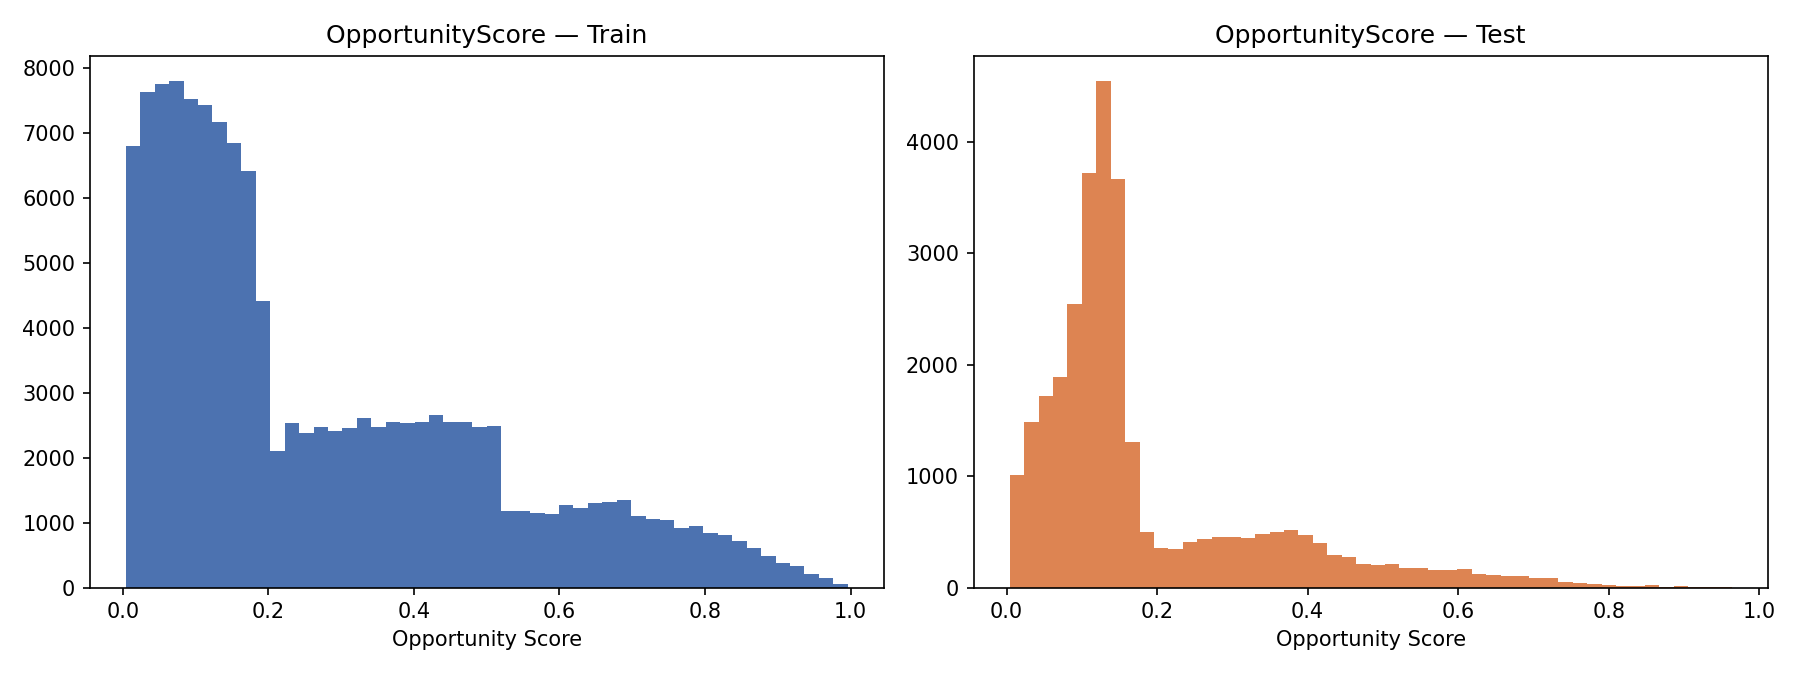
\includegraphics[width=\textwidth]{target_distribution.png}
    \caption{Distribution of the Reference Opportunity Score in the Training and Test Datasets}
    \label{fig:target_distribution}
\end{figure}

The Opportunity Score distribution differs between the training and test datasets. The training set shows a broader range of scores, including a visible proportion above $0.5$, while the test set is more concentrated in the lower range, particularly around $0.05$--$0.20$. The test set also has a thinner upper tail. This difference is consistent with the client-grouped splitting strategy, where the test set contains client groups not used during training. Thus, the final evaluation was performed under a distribution that differs from the training data. The shift is not treated as an error but as an important factor when interpreting model performance. The higher concentration of lower scores in the test set also indicates that high-opportunity observations form a relatively selective subset of the data.

This distribution supports the use of ranking metrics such as \textbf{Precision@K}, \textbf{NDCG@K}, and \textbf{Spearman Rank Correlation}, which evaluate both overall ordering and the ability to prioritize higher-opportunity observations. Overall, the analysis confirms that the Opportunity Score provides a continuous reference for ranking content records, while the observed distribution shift highlights the challenge of generalizing across unseen client groups. The following sections therefore examine the dataset split characteristics, baseline performance, and comparative model results.

\section{\textit{Data Split Analysis}}

The dataset was divided into training, validation, and test partitions using a \textbf{client-grouped splitting strategy}. Unlike a conventional row-wise split, the pseudonymized client identifier was used for grouping, ensuring that all observations from a client remained within a single partition. The final split contained \textbf{54 clients} and \textbf{205,749 observations}. The training, validation, and test partitions contained \textbf{42, 5, and 7 clients}, respectively. The distribution of observations is summarized in Table~\ref{tab:data_split_analysis}.

\begin{table}[htbp]
\centering
\caption{Final Client-Grouped Data Split}
\label{tab:data_split_analysis}
\begin{tabular}{|l|r|r|r|}
\hline
\textbf{Split} & \textbf{Observations} & \textbf{Clients} & \textbf{Percentage} \\
\hline
Training & 143,979 & 42 & 69.98\% \\
\hline
Validation & 30,945 & 5 & 15.04\% \\
\hline
Test & 30,825 & 7 & 14.98\% \\
\hline
\textbf{Total} & \textbf{205,749} & \textbf{54} & \textbf{100.00\%} \\
\hline
\end{tabular}
\end{table}

An overlap check was performed after splitting to verify client-level separation. No client appeared in more than one partition, confirming that the grouping constraint was maintained. This strategy reduced the risk of client-specific patterns being learned during training and encountered again during evaluation. The final test set therefore represented client groups not used during model development, providing a more realistic assessment of generalization. After constructing the Opportunity Score, observations without valid target values were excluded from the respective modelling stages. The resulting valid-target counts are presented in Table~\ref{tab:valid_target_split_analysis}.

\begin{table}[htbp]
\centering
\caption{Valid Opportunity Score Observations After Target Filtering}
\label{tab:valid_target_split_analysis}
\begin{tabular}{|l|r|r|r|}
\hline
\textbf{Split} & \textbf{Original Rows} & \textbf{Valid Target Rows} & \textbf{Excluded (\%)} \\
\hline
Training & 143,979 & 130,383 & 9.44\% \\
\hline
Validation & 30,945 & 30,557 & 1.25\% \\
\hline
Test & 30,825 & 30,532 & 0.95\% \\
\hline
\end{tabular}
\end{table}
The training partition experienced the largest reduction after target filtering, with \textbf{13,596 observations} excluded. In comparison, only \textbf{388 validation} and \textbf{293 test} observations were excluded. Because the split was performed at the client level, the partitions were not forced to contain identical numbers of observations. The primary objective was to maintain client independence while preserving the natural distribution of records across clients. The final split provided three distinct roles: training data for learning the relationship between features and the Opportunity Score, validation data for candidate model comparison and selection, and test data for the final comparison between HistGradientBoosting and the Age-Based Baseline. Since the test clients were not observed during training, differences between validation and test performance also provide context for evaluating generalization across client groups.

\section{\textit{Baseline Scoring Results}}

Before evaluating the machine learning models, the Age-Based Baseline was used as a transparent reference. It ranked observations using \texttt{content\_age\_days}, with older content receiving higher priority according to its age percentile derived from the training data. The baseline required no model training, hyperparameter tuning, or additional input variables. Its purpose was to provide a simple and reproducible reference for evaluating the machine learning approaches. The Age-Based Baseline was evaluated on the validation dataset using the same ranking metrics as the machine learning models. The results are presented in Table~\ref{tab:age_baseline_validation}.

\begin{table}[htbp]
\centering
\caption{Validation Performance of the Age-Based Baseline}
\label{tab:age_baseline_validation}
\begin{tabular}{|l|c|}
\hline
\textbf{Metric} & \textbf{Age-Based Baseline} \\
\hline
Spearman Rank Correlation & 0.4349 \\
\hline
NDCG@1\% & 0.1970 \\
\hline
Precision@1\% & 0.0131 \\
\hline
NDCG@5\% & 0.3009 \\
\hline
Precision@5\% & 0.0870 \\
\hline
NDCG@10\% & 0.4774 \\
\hline
Precision@10\% & 0.2615 \\
\hline
\end{tabular}
\end{table}

The validation results show that content age provided useful ranking information. The Age-Based Baseline achieved a \textbf{Spearman Rank Correlation of 0.4349}, indicating a moderate positive relationship with the reference Opportunity Score. Performance varied across ranking cutoffs. Precision@1\% was \textbf{0.0131}, increasing to \textbf{0.2615} at the 10\% cutoff. Similarly, NDCG increased from \textbf{0.1970} at 1\% to \textbf{0.3009} at 5\% and \textbf{0.4774} at 10\%. The baseline achieved the highest Precision@10\% among the validation approaches, showing that the simple age-based ranking remained competitive when a broader top 10\% of records was considered. These results demonstrate the importance of including a transparent baseline in the evaluation. Machine learning models therefore needed to demonstrate measurable ranking improvements beyond the information provided by content age alone. The Age-Based Baseline was retained for the final evaluation. After selecting HistGradientBoosting using validation performance, both approaches were evaluated on the held-out test clients to assess their ranking performance under previously unseen client conditions.

\section{\textit{Candidate Model Comparison}}
Candidate models were compared on the validation dataset to identify the most suitable approach before final test evaluation. The comparison included ElasticNet Regression, Random Forest, Histogram-Based Gradient Boosting (HistGB), XGBoost, and LightGBM, along with the Age-Based Baseline as a reference. All approaches were evaluated using the same validation data and ranking framework. The comparison used Spearman Rank Correlation, Precision@K, and NDCG@K at the $1\%$, $5\%$, and $10\%$ ranking cutoffs. The validation results are presented in Table~\ref{tab:candidate_model_comparison}.

\begin{table}[htbp]
\centering
\caption{Comparison of Candidate Models on the Validation Dataset}
\label{tab:candidate_model_comparison}
\resizebox{\textwidth}{!}{
\begin{tabular}{|l|c|c|c|c|c|c|c|}
\hline
\textbf{Model} &
\textbf{Spearman} &
\textbf{NDCG@1\%} &
\textbf{Precision@1\%} &
\textbf{NDCG@5\%} &
\textbf{Precision@5\%} &
\textbf{NDCG@10\%} &
\textbf{Precision@10\%} \\
\hline
ElasticNet &
0.4938 &
0.4507 &
0.0490 &
0.4565 &
0.1453 &
0.4959 &
0.2065 \\
\hline
Random Forest &
0.4286 &
0.3951 &
0.0131 &
0.4243 &
0.1027 &
0.4805 &
0.2137 \\
\hline
HistGB &
0.4661 &
\textbf{0.5282} &
\textbf{0.1176} &
\textbf{0.5269} &
\textbf{0.2186} &
\textbf{0.5350} &
0.2471 \\
\hline
XGBoost &
0.4510 &
0.4848 &
0.0654 &
0.4945 &
0.1682 &
0.5216 &
0.2317 \\
\hline
LightGBM &
0.4265 &
0.3985 &
0.0621 &
0.4637 &
0.1597 &
0.5032 &
0.2212 \\
\hline
Age Baseline &
0.4349 &
0.1970 &
0.0131 &
0.3009 &
0.0870 &
0.4774 &
\textbf{0.2615} \\
\hline
\end{tabular}
}
\end{table}

The results show that no single approach achieved the highest performance across all evaluation metrics. However, Histogram-Based Gradient Boosting (HistGB) showed the strongest performance for the defined model selection criterion. HistGB achieved the highest NDCG@1\% of 0.5282, Precision@1\% of 0.1176, NDCG@5\% of 0.5269, Precision@5\% of 0.2186, and NDCG@10\% of 0.5350. The predefined selection criterion was validation NDCG@5\%. HistGB achieved the highest value of 0.5269 among the candidate models and was therefore selected as the final machine learning model. ElasticNet achieved the highest Spearman Rank Correlation of 0.4938, indicating the strongest overall monotonic agreement with the reference ranking. However, its top-$K$ performance was lower than HistGB. XGBoost also showed competitive performance, with NDCG@5\% of 0.4945 and NDCG@10\% of 0.5216. LightGBM produced moderate results but did not exceed HistGB on the selection criterion. Random Forest showed lower performance at the narrower cutoffs. Its Precision@1\% was 0.0131 compared with 0.1176 for HistGB. The Age-Based Baseline remained competitive at broader cutoffs and achieved the highest Precision@10\% of 0.2615. This highlights the importance of comparing machine learning models with a simple and transparent baseline. Overall, HistGB was particularly effective at prioritizing higher-opportunity observations near the top of the ranking. Since validation NDCG@5\% was the predefined selection criterion, its highest value on this metric led to its selection as the final model. The selected HistGB model was subsequently evaluated on the unseen test dataset and compared with the Age-Based Baseline to assess whether its validation performance generalized to unseen client groups.

\section{\textit{Validation Performance Analysis}}
The validation stage was used to compare the candidate machine learning models and select the final model before evaluation on the held-out test dataset. The objective was to assess their ability to rank content records according to the reference Opportunity Score. The models were evaluated using Spearman Rank Correlation, Precision@K, and NDCG@K at ranking cutoffs of 1\%, 5\%, and 10\%. Since performance varied across metrics and ranking cutoffs, model selection followed the predefined primary criterion of NDCG@5\%. The validation results are summarized in Table~\ref{tab:validation_performance_analysis}.

\begin{table}[htbp]
\centering
\caption{Validation Performance Analysis of Candidate Models}
\label{tab:validation_performance_analysis}
\resizebox{\textwidth}{!}{
\begin{tabular}{|l|c|c|c|c|c|c|c|}
\hline
\textbf{Model} &
\textbf{Spearman} &
\textbf{NDCG@1\%} &
\textbf{Precision@1\%} &
\textbf{NDCG@5\%} &
\textbf{Precision@5\%} &
\textbf{NDCG@10\%} &
\textbf{Precision@10\%} \\
\hline
ElasticNet &
0.4938 &
0.4507 &
0.0490 &
0.4565 &
0.1453 &
0.4959 &
0.2065 \\
\hline
Random Forest &
0.4286 &
0.3951 &
0.0131 &
0.4243 &
0.1027 &
0.4805 &
0.2137 \\
\hline
HistGB &
0.4661 &
\textbf{0.5282} &
\textbf{0.1176} &
\textbf{0.5269} &
\textbf{0.2186} &
\textbf{0.5350} &
0.2471 \\
\hline
XGBoost &
0.4510 &
0.4848 &
0.0654 &
0.4945 &
0.1682 &
0.5216 &
0.2317 \\
\hline
LightGBM &
0.4265 &
0.3985 &
0.0621 &
0.4637 &
0.1597 &
0.5032 &
0.2212 \\
\hline
Age Baseline &
0.4349 &
0.1970 &
0.0131 &
0.3009 &
0.0870 &
0.4774 &
\textbf{0.2615} \\
\hline
\end{tabular}
}
\end{table}
HistGradientBoosting achieved the highest value on the predefined selection criterion, with a validation NDCG@5\% of 0.5269. This exceeded the corresponding values of XGBoost, LightGBM, Random Forest, ElasticNet Regression, and the Age-Based Baseline.HistGB also achieved the highest NDCG@1\%, Precision@1\%, Precision@5\%, and NDCG@10\%. These results indicate strong performance in prioritizing higher-opportunity observations near the top of the ranking.

However, HistGB did not lead on every metric. ElasticNet achieved the highest Spearman Rank Correlation of 0.4938, compared with 0.4661 for HistGB, indicating stronger overall monotonic agreement with the reference ranking. The Age-Based Baseline remained competitive at the 10\% cutoff, achieving the highest Precision@10\% of 0.2615. This shows that content age alone provided substantial ranking information in the validation data. Therefore, model performance depended on the selected evaluation criterion. In this project, NDCG@5\% was used as the primary criterion because the objective was to prioritize relevant observations within the top 5\% of the ranked output. Based on this criterion, HistGradientBoosting was selected as the final machine learning model. It was then evaluated on the held-out test dataset and compared with the Age-Based Baseline on previously unseen client groups. Thus, the validation analysis supported HistGB under the predefined selection objective while also demonstrating the importance of comparing alternative models and a simple baseline. The final test evaluation was required to assess whether the validation results generalized to unseen client data.

\section{\textit{Final Test Evaluation: HistGB vs.\ Age Baseline}}

Following model selection, HistGradientBoosting was evaluated on the held-out test dataset and compared with the Age-Based Baseline. The test set contained observations from client groups not used during training or validation, providing the final assessment of generalization to unseen clients.

The evaluation used \textbf{30,532 observations} with valid Opportunity Score values. Both approaches were evaluated on the same test observations using Spearman Rank Correlation, Precision@K, and NDCG@K.

The final test results are presented in Table~\ref{tab:final_test_histgb_vs_baseline}.

\begin{table}[htbp]
\centering
\caption{Final Test Performance: HistGB versus Age-Based Baseline}
\label{tab:final_test_histgb_vs_baseline}
\resizebox{\textwidth}{!}{
\begin{tabular}{|l|c|c|c|c|c|c|c|}
\hline
\textbf{Method} &
\textbf{Spearman} &
\textbf{NDCG@1\%} &
\textbf{Precision@1\%} &
\textbf{NDCG@5\%} &
\textbf{Precision@5\%} &
\textbf{NDCG@10\%} &
\textbf{Precision@10\%} \\
\hline
HistGB &
\textbf{0.1556} &
\textbf{0.1735} &
0.0163 &
0.3363 &
0.1094 &
\textbf{0.3744} &
0.1703 \\
\hline
Age Baseline &
0.0283 &
0.1642 &
0.0163 &
\textbf{0.3479} &
\textbf{0.1421} &
0.3717 &
\textbf{0.1762} \\
\hline
\end{tabular}
}
\end{table}

The final test results show a more balanced outcome than the validation results, with HistGB not outperforming the Age-Based Baseline on every metric. HistGB achieved a Spearman Rank Correlation of 0.1556, compared with 0.0283 for the baseline, indicating stronger overall agreement with the reference ranking. HistGB also achieved higher NDCG@1\% and NDCG@10\%, with values of 0.1735 and 0.3744, respectively, compared with 0.1642 and 0.3717 for the baseline.

At the 1\% cutoff, both approaches achieved the same Precision@1\% of 0.0163. Thus, neither approach showed an advantage in the proportion of relevant observations within the top 1\%. The Age-Based Baseline performed better at the 5\% cutoff, achieving NDCG@5\% of 0.3479 and Precision@5\% of 0.1421, compared with 0.3363 and 0.1094 for HistGB. The baseline also achieved a higher Precision@10\% of 0.1762 compared with 0.1703 for HistGB.

These results show that the validation advantage of HistGB did not generalize uniformly across all metrics on unseen client groups. HistGB achieved higher Spearman correlation and NDCG at the 1\% and 10\% cutoffs, while the Age-Based Baseline performed better on NDCG@5\%, Precision@5\%, and Precision@10\%. Figure~\ref{fig:baseline_vs_model} provides a visual comparison of HistGB and the Age-Based Baseline across the evaluation metrics.

\begin{figure}[htbp]
    \centering
    \includegraphics[width=\textwidth]{baseline_vs_model.png}
    \caption{Comparison of Final Test Performance Between HistGB and the Age-Based Baseline}
    \label{fig:baseline_vs_model}
\end{figure}

The final results are important in relation to the project's objective. The machine learning component was intended to determine whether combining multiple content and structural features could provide additional value for ranking content opportunities, rather than only improving numerical prediction over the baseline. The test evaluation shows that HistGB provided additional value in overall rank correlation and selected NDCG metrics. However, its greater complexity did not consistently improve top-$K$ ranking performance.

The strong performance of the Age-Based Baseline indicates that \texttt{content\_age\_days} remained an informative ranking signal. This is also supported by the feature importance analysis, where it was identified as the most influential feature in HistGB. Overall, HistGB improved certain aspects of ranking performance, particularly overall rank agreement, while the Age-Based Baseline remained competitive and performed better at several top-$K$ cutoffs.

These findings highlight the importance of retaining a transparent baseline throughout the evaluation. The results do not indicate that machine learning consistently outperformed the baseline; instead, performance varied with the evaluation metric and ranking cutoff. Thus, the final evaluation provides a realistic assessment of the system. HistGB demonstrated value for selected ranking objectives, but it did not consistently outperform the simpler Age-Based Baseline across all evaluation measures.

\section{\textit{Ranking Performance Analysis}}

The final evaluation focused on the ranking quality of the selected Histogram-Based Gradient Boosting model and the Age-Based Baseline. Since the system is intended to prioritize content records for human review, the placement of relevant observations near the top of the ranking is important. Ranking performance was evaluated using Precision@K, Normalized Discounted Cumulative Gain at K (NDCG@K), and Spearman Rank Correlation. Each metric provides a different view of ranking quality.

Precision@K measures the proportion of relevant observations within the top $K$ portion of the ranking. NDCG@K considers both relevance and position, giving greater importance to relevant observations appearing near the top. Spearman Rank Correlation measures overall agreement between the predicted and reference Opportunity Score rankings. The final ranking performance results are summarized in Table~\ref{tab:ranking_performance_summary}.

\begin{table}[htbp]
\centering
\caption{Final Ranking Performance on the Test Dataset}
\label{tab:ranking_performance_summary}
\resizebox{\textwidth}{!}{
\begin{tabular}{|l|c|c|c|c|c|c|c|}
\hline
\textbf{Method} &
\textbf{Spearman} &
\textbf{NDCG@1\%} &
\textbf{Precision@1\%} &
\textbf{NDCG@5\%} &
\textbf{Precision@5\%} &
\textbf{NDCG@10\%} &
\textbf{Precision@10\%} \\
\hline
HistGB &
\textbf{0.1556} &
\textbf{0.1735} &
0.0163 &
0.3363 &
0.1094 &
\textbf{0.3744} &
0.1703 \\
\hline
Age Baseline &
0.0283 &
0.1642 &
0.0163 &
\textbf{0.3479} &
\textbf{0.1421} &
0.3717 &
\textbf{0.1762} \\
\hline
\end{tabular}
}
\end{table}
The ranking results show that neither approach consistently dominated across all evaluation measures. HistGB achieved the higher Spearman Rank Correlation of 0.1556 compared with 0.0283 for the Age-Based Baseline, indicating stronger overall agreement with the reference Opportunity Score ranking. At the 1\% cutoff, HistGB achieved a slightly higher NDCG@1\% of 0.1735 compared with 0.1642, while both approaches recorded the same Precision@1\% of 0.0163.

At the 5\% cutoff, the Age-Based Baseline performed better, with NDCG@5\% of 0.3479 and Precision@5\% of 0.1421, compared with 0.3363 and 0.1094 for HistGB. At the 10\% cutoff, HistGB achieved a slightly higher NDCG@10\% of 0.3744 compared with 0.3717, whereas the baseline achieved higher Precision@10\% of 0.1762 compared with 0.1703.

Thus, performance depended on both the evaluation metric and ranking cutoff. HistGB showed stronger overall rank correlation and NDCG at the 1\% and 10\% cutoffs, while the Age-Based Baseline performed better on NDCG@5\%, Precision@5\%, and Precision@10\%. These results highlight the importance of using multiple ranking metrics. Spearman Rank Correlation alone would not capture the differences observed in top-$K$ performance, where the baseline remained competitive and performed better at several cutoffs.

Therefore, the results do not indicate universal superiority of the machine learning model. Instead, HistGB and the Age-Based Baseline showed different performance characteristics across the ranking measures. The following subsections analyse Precision@K, NDCG@K, and Spearman Rank Correlation individually to provide a more detailed view of the ranking behaviour.

\subsection{\textit{Precision@K Analysis}}
Precision@K was used to measure the proportion of relevant observations within the top-ranked portion of the test dataset. This metric is important because the system is designed to support human review, where reviewers may focus on the highest-priority records rather than the complete dataset. The Precision@K results for HistGradientBoosting and the Age-Based Baseline are presented in Table~\ref{tab:precision_at_k_results}.

\begin{table}[htbp]
\centering
\caption{Precision@K Performance on the Final Test Dataset}
\label{tab:precision_at_k_results}
\begin{tabular}{|l|c|c|c|}
\hline
\textbf{Method} & \textbf{Precision@1\%} & \textbf{Precision@5\%} & \textbf{Precision@10\%} \\
\hline
HistGB & 0.0163 & 0.1094 & 0.1703 \\
\hline
Age Baseline & 0.0163 & \textbf{0.1421} & \textbf{0.1762} \\
\hline
\end{tabular}
\end{table}
At the 1\% cutoff, both HistGB and the Age-Based Baseline achieved a Precision@1\% of 0.0163. Thus, neither approach showed an advantage in identifying relevant observations within the top 1\% of the test ranking. At the 5\% cutoff, the Age-Based Baseline performed better, achieving Precision@5\% of 0.1421 compared with 0.1094 for HistGB. This indicates that the baseline identified a higher proportion of relevant observations within the top 5\%. At the 10\% cutoff, the baseline again achieved higher precision, with a Precision@10\% of 0.1762 compared with 0.1703 for HistGB. The difference between the approaches was relatively small. Figure~\ref{fig:precision_at_k} provides a visual comparison of Precision@K across the three evaluation cutoffs.

\begin{figure}[htbp]
    \centering
    \includegraphics[width=\textwidth]{precision_at_k.png}
    \caption{Precision@K Comparison Between HistGB and the Age-Based Baseline}
    \label{fig:precision_at_k}
\end{figure}

The Precision@K results show that the Age-Based Baseline was more effective at concentrating relevant observations within the broader top-ranked portions of the test dataset. HistGB matched the baseline at 1\% but did not exceed it at the 5\% or 10\% cutoffs. This is relevant to the practical use of the system, where a subset of content records may be selected for human review. At the 5\% and 10\% cutoffs, the Age-Based Baseline produced higher precision on the held-out test dataset.

Although HistGB was selected during validation based on its higher NDCG@5\%, the final Precision@K results show that this advantage did not consistently translate into higher precision on unseen client groups. Overall, the results indicate that content age remained an informative signal for prioritizing relevant observations. The additional features used by HistGB did not consistently improve the concentration of relevant records within the top-ranked recommendations.

\subsection{\textit{NDCG@K Analysis}}

Normalized Discounted Cumulative Gain at $K$, denoted as NDCG@K, was used to evaluate ranking quality while considering the positions of relevant observations. Unlike Precision@K, NDCG@K gives greater importance to relevant observations appearing closer to the top of the ranking. The NDCG@K results for HistGradientBoosting and the Age-Based Baseline are presented in Table~\ref{tab:ndcg_at_k_results}.

\begin{table}[htbp]
\centering
\caption{NDCG@K Performance on the Final Test Dataset}
\label{tab:ndcg_at_k_results}
\begin{tabular}{|l|c|c|c|}
\hline
\textbf{Method} & \textbf{NDCG@1\%} & \textbf{NDCG@5\%} & \textbf{NDCG@10\%} \\
\hline
HistGB & \textbf{0.1735} & 0.3363 & \textbf{0.3744} \\
\hline
Age Baseline & 0.1642 & \textbf{0.3479} & 0.3717 \\
\hline
\end{tabular}
\end{table}

At the 1\% cutoff, HistGB achieved an NDCG@1\% of 0.1735, slightly higher than the Age-Based Baseline value of 0.1642. This indicates a marginally better ordering of relevant observations within the top 1\%. At the 5\% cutoff, the Age-Based Baseline performed better, with an NDCG@5\% of 0.3479 compared with 0.3363 for HistGB. At the 10\% cutoff, HistGB again showed a marginal advantage, achieving an NDCG@10\% of 0.3744 compared with 0.3717 for the baseline. Figure~\ref{fig:ndcg_comparison} presents the NDCG results across the three ranking cutoffs.

\begin{figure}[htbp]
    \centering
    \includegraphics[width=\textwidth]{ndcg_comparison.png}
    \caption{NDCG@K Comparison Between HistGB and the Age-Based Baseline}
    \label{fig:ndcg_comparison}
\end{figure}

The NDCG@K results show that the relative performance of HistGB and the Age-Based Baseline varied across ranking cutoffs. HistGB achieved slightly higher NDCG at 1\% and 10\%, while the baseline achieved the higher value at 5\%. The differences were relatively small across the evaluated cutoffs, indicating that neither approach consistently dominated. HistGB provided some improvement in ranking order at specific ranges, while the simpler age-based approach remained competitive.

HistGB was selected during validation using NDCG@5\% as the primary criterion. However, its higher validation performance at this cutoff did not persist on the held-out test data for unseen client groups. These results highlight the importance of separate test evaluation. While validation results indicated an advantage for HistGB under the selection criterion, the test results show that its relative performance depended on the ranking range considered.

\subsection{\textit{Spearman Rank Correlation Analysis}}

Spearman Rank Correlation was used to measure the overall monotonic relationship between the rankings generated by each method and the reference Opportunity Score ranking. Unlike Precision@K and NDCG@K, it evaluates ranking agreement across the complete test dataset. The final Spearman Rank Correlation results are presented in Table~\ref{tab:spearman_results}.

\begin{table}[htbp]
\centering
\caption{Spearman Rank Correlation on the Final Test Dataset}
\label{tab:spearman_results}
\begin{tabular}{|l|c|}
\hline
\textbf{Method} & \textbf{Spearman Rank Correlation} \\
\hline
HistGB & \textbf{0.1556} \\
\hline
Age Baseline & 0.0283 \\
\hline
\end{tabular}
\end{table}

The HistGradientBoosting model achieved a Spearman Rank Correlation of 0.1556, compared with 0.0283 for the Age-Based Baseline. Thus, HistGB showed stronger overall monotonic agreement with the reference Opportunity Score ranking across the held-out test dataset. Although both correlation values were relatively low, the difference indicates that the multiple content, structural, and categorical features used by HistGB captured more of the overall ranking relationship than \texttt{content\_age\_days} alone.

The Age-Based Baseline remained competitive on several Precision@K and NDCG@K measures but showed weaker agreement with the complete reference ranking. This suggests that content age was useful for identifying some higher-priority observations but less effective for reproducing the overall Opportunity Score ordering. The Spearman results therefore highlight a key strength of HistGB: it produced a ranking more closely aligned with the overall reference ranking, even though it did not consistently outperform the baseline at every top-$K$ cutoff.

This difference also reflects the complementary nature of the evaluation metrics. Precision@K and NDCG@K focus on selected portions of the ranking, whereas Spearman Rank Correlation evaluates ranking agreement across all observations. Overall, HistGB provided additional value in modelling the overall Opportunity Score ranking, while the Age-Based Baseline remained competitive at specific top-$K$ cutoffs. This supports the use of multiple metrics when evaluating the proposed ranking system.

\section{\textit{Feature Importance Analysis}}

Feature importance analysis was performed to examine the input variables most relied upon by the selected HistGradientBoosting model when generating Opportunity Score predictions. Permutation importance was calculated using the validation dataset. Permutation importance measures the change in model performance after randomly shuffling a feature. A larger performance decrease indicates greater model reliance on that feature. Values near zero indicate limited contribution, while negative values may indicate limited usefulness or noise under the evaluated setting. Figure~\ref{fig:feature_importance} presents the permutation feature importance results for the selected HistGradientBoosting model.

\begin{figure}[htbp]
    \centering
    \includegraphics[width=\textwidth]{feature_importance.png}
    \caption{Permutation Feature Importance for the HistGradientBoosting Model}
    \label{fig:feature_importance}
\end{figure}

The results show that \texttt{content\_age\_days} was the dominant feature in the HistGradientBoosting model. Its permutation importance was substantially higher than that of the other variables, indicating strong model reliance on content age. The second strongest feature was \texttt{main\_intent\_informational}, suggesting that search intent provided additional information beyond content age. The remaining features had considerably smaller importance values. Although they may have contributed to individual predictions or feature interactions, their overall contribution to validation performance was lower than that of content age and informational intent.

Some features had importance values close to zero, while one showed a small negative value. These results were retained because they provide information about feature usefulness. A negative permutation importance indicates that shuffling the feature slightly improved validation performance, suggesting limited useful information or mild noise under the evaluated configuration.

The dominance of \texttt{content\_age\_days} is consistent with the strong performance of the Age-Based Baseline, which uses the same feature. This helps explain why the simple baseline remained competitive during the final test evaluation. Although HistGB incorporated multiple content, structural, and categorical features, its strongest signal remained content age. Consequently, the additional model complexity did not produce consistent improvements across all ranking metrics.

The importance of \texttt{main\_intent\_informational} also shows that HistGB captured information beyond content age. However, the comparatively low importance of the remaining features indicates that their overall contribution was limited under the evaluated model configuration. It is important to note that permutation importance measures \textit{model reliance}, not causal influence. Therefore, these results do not imply that changing content age or search intent would directly change the Opportunity Score. They only indicate how strongly the trained HistGradientBoosting model relied on these variables when generating predictions for the available dataset.

Overall, the feature importance analysis highlights three main findings:

\begin{enumerate}
    \item \texttt{content\_age\_days} was the dominant feature in the HistGradientBoosting model;

    \item \texttt{main\_intent\_informational} was the second strongest feature;

    \item most remaining features had substantially lower importance.
\end{enumerate}

These findings help explain why the Age-Based Baseline remained competitive on unseen test clients. HistGB captured additional relationships through multiple features, contributing to its higher Spearman Rank Correlation. However, the dominance of content age allowed the simpler baseline to remain competitive on several top-$K$ metrics. Thus, the feature importance analysis connects the model's feature reliance with the comparative results observed during the final test evaluation.

\section{\textit{Predicted vs.\ Reference Opportunity Score}}
The relationship between the predicted Opportunity Scores from HistGradientBoosting and the reference Opportunity Scores was examined using the final ranking results. The analysis assessed whether the model could capture the reference ordering for previously unseen client groups. HistGB achieved a Spearman Rank Correlation of 0.1556 on the test dataset. This indicates a positive relationship between the predicted and reference rankings, although the relatively low value shows that the model did not reproduce the complete ordering of the reference scores.

Since the objective was ranking rather than exact score prediction, the model was evaluated using ranking-oriented metrics in addition to Spearman correlation. HistGB showed stronger overall ranking agreement than the Age-Based Baseline, which achieved a Spearman Rank Correlation of 0.0283. This suggests that combining multiple input features captured more of the ranking relationship represented by the Opportunity Score. However, the higher overall correlation did not translate into consistent superiority across all top-$K$ metrics. The Age-Based Baseline performed better on NDCG@5\%, Precision@5\%, and Precision@10\%. Overall, the analysis shows that HistGradientBoosting captured useful aspects of the Opportunity Score ordering but did not consistently outperform the simpler baseline across all ranking objectives.

This finding reinforces the use of multiple evaluation metrics. Spearman Rank Correlation measures agreement across the complete ranking, while Precision@K and NDCG@K focus more directly on the placement of higher-priority observations within the top-ranked portion.

\section{\textit{Train vs.\ Test Opportunity Score Distribution}}
The Opportunity Score distributions across the training and test datasets were considered when interpreting the final model performance. The training data showed a broader range of scores, while the test data was more concentrated in the lower Opportunity Score range. This difference is relevant because the model was trained on one group of clients and evaluated on completely unseen test clients. Since the split was performed at the client level, the test distribution was not expected to exactly match the training distribution.

The difference represents a form of distribution shift. HistGradientBoosting learned relationships between the selected features and Opportunity Score from the training clients and applied them to test clients with different data characteristics. This also provides context for the difference between validation and test performance. HistGB achieved the highest validation NDCG@5\%, which was the predefined model selection criterion, but the Age-Based Baseline achieved a higher NDCG@5\% on the held-out test clients.

This change shows that the relationships learned from the development clients did not transfer uniformly to the unseen clients. It does not invalidate the validation process; rather, it demonstrates the importance of using a separate test dataset to assess generalization. The client-grouped split also provided a more challenging evaluation than a random row-wise split. A row-wise split could place observations from the same clients in both training and test sets, potentially producing more optimistic results. Separating clients reduced this possibility.

Therefore, the difference between the training and test Opportunity Score distributions should be considered when interpreting the final results. The mixed performance of HistGB and the Age-Based Baseline reflects both their modelling characteristics and the challenge of generalizing across previously unseen client groups.

\section{\textit{Recommendation and Reason Code Analysis}}
The final stage converted the model output into a ranked recommendation framework for human review. The objective was to demonstrate how predicted Opportunity Scores could be used to prioritize content records for further examination. The selected HistGradientBoosting model generated an Opportunity Score for each eligible record. These scores were sorted in descending order, assigning higher priority to records with higher predicted scores.

The ranked output was designed as a \textbf{decision-support mechanism}, not an automated decision-making system. The system prioritizes records for review, while final interpretation and action remain with human reviewers. Reason codes were included to provide human-readable context for the generated recommendations. Since the numerical Opportunity Score alone does not explain the prioritization of a record, these codes provide additional information about the characteristics associated with its ranking.

Reason codes must be interpreted as descriptive rather than causal. They reflect available data signals and the defined recommendation logic but do not imply that changing a particular characteristic will directly improve real-world content performance. The recommendation framework therefore separates ranking from decision-making. The model generates the prioritized list, while human reviewers determine whether a record requires further investigation or action. This human-in-the-loop approach is intended to reduce the effort required to identify potentially important records within a large content collection without replacing human judgment.

The final system output consists of three main components:

\begin{enumerate}
    \item \textbf{Predicted Opportunity Scores:} Scores generated by the selected HistGradientBoosting model;

    \item \textbf{Priority Ranking:} Content records ordered according to their predicted scores; and

    \item \textbf{Reason Codes:} Descriptive information supporting interpretation of the recommendations.
\end{enumerate}

Overall, the framework connects the machine learning pipeline with its intended practical use. It provides a reproducible method for prioritizing content records and supporting human reviewers in identifying observations that may warrant further attention.

\section{\textit{Discussion of Results}}
The experimental results show that both HistGradientBoosting and the Age-Based Baseline captured useful ranking information, but their performance varied across metrics and datasets. During validation, HistGB achieved the highest NDCG@5\% of 0.5269, the predefined model selection criterion, and was therefore selected as the final model. It also achieved the highest NDCG@1\%, NDCG@10\%, Precision@1\%, and Precision@5\%, while ElasticNet achieved the highest Spearman Rank Correlation and the Age-Based Baseline achieved the highest Precision@10\%.

On the held-out test dataset, HistGB achieved a higher Spearman Rank Correlation (0.1556 vs.\ 0.0283) and slightly higher NDCG@1\% and NDCG@10\%. The Age-Based Baseline, however, achieved higher NDCG@5\%, Precision@5\%, and Precision@10\%, while both methods achieved the same Precision@1\% of 0.0163. Feature importance analysis identified \texttt{content\_age\_days} as the dominant feature, helping explain the strong performance of the Age-Based Baseline. The difference between validation and test results also indicates that HistGB's advantage did not generalize uniformly to unseen client groups.

Overall, the results demonstrate that HistGB provided stronger overall ranking agreement and performed well under the predefined validation criterion, but it did not consistently outperform the simpler baseline across all test metrics. The findings therefore support the use of multiple ranking measures and transparent baseline comparison when assessing the proposed system.

%----------------------------------------------------------------------
\chapter{CONCLUSIONS \& FUTURE SCOPE}

\section{\textit{Conclusion}}

This project developed and evaluated a machine learning-based content opportunity ranking system using content, search, and structural signals. The objective was to determine whether supervised machine learning could provide additional value over a simple Age-Based Baseline for prioritizing content records. A complete workflow was implemented covering data preparation, exploratory analysis, preprocessing, feature selection, Opportunity Score construction, client-grouped splitting, model development, evaluation, and recommendation generation. The client-grouped split ensured that the final test set contained previously unseen client groups.

The Age-Based Baseline used \texttt{content\_age\_days}, while ElasticNet Regression, Random Forest, HistGradientBoosting, XGBoost, and LightGBM were evaluated as candidate models. HistGradientBoosting was selected using the predefined validation NDCG@5\% criterion, achieving a value of 0.5269. On the held-out test dataset, HistGB achieved a higher Spearman Rank Correlation of 0.1556 compared with 0.0283 for the Age-Based Baseline, along with slightly higher NDCG at the 1\% and 10\% cutoffs. However, the baseline achieved higher NDCG@5\%, Precision@5\%, and Precision@10\%, showing that HistGB did not consistently outperform the simpler approach.

Feature importance analysis identified \texttt{content\_age\_days} as the dominant feature in HistGB. This helps explain the strong performance of the Age-Based Baseline and shows that additional features did not consistently improve top-$K$ ranking performance. Overall, the results demonstrate that machine learning can provide useful information for content opportunity ranking, particularly in overall ranking agreement. However, the findings do not support universal superiority of the more complex model. The comparative performance depended on the evaluation metric, ranking cutoff, and generalization to unseen client groups.

The project also demonstrated a reproducible recommendation framework in which predicted scores are converted into ranked outputs and supported by reason codes for human review. The system therefore functions as a decision-support tool rather than an automated decision-making system. In conclusion, the project highlights the importance of transparent baselines, client-grouped evaluation, multiple ranking metrics, and separate test data when assessing machine learning-based ranking systems.

\section{\textit{Limitations of the Project}}
Although the project successfully developed and evaluated a machine learning-based framework for content opportunity prioritization, several limitations should be considered.

First, the dataset contained 54 pseudonymized clients. While client-grouped splitting provided a stronger generalization assessment than random row-wise splitting, this number of client groups may not capture the full diversity of content and search behaviour found in broader real-world settings. 

Second, the training and test datasets showed different Opportunity Score distributions, with the test set more concentrated in the lower score range. This distribution shift may have contributed to the differences between validation and final test performance.

Another limitation concerns the Opportunity Score itself. It is a constructed reference target based on available search-related signals rather than an independently observed business outcome. Therefore, the models evaluate their ability to reproduce this defined ranking objective rather than directly predict outcomes such as traffic, conversions, or improvements after content changes. The available feature set also limited the modelling capability. Although multiple content, structural, and categorical features were used, \texttt{content\_age\_days} remained the dominant feature in HistGB. The relatively smaller contribution of other features may explain why the machine learning approach did not consistently outperform the Age-Based Baseline.

The evaluation was primarily based on offline ranking metrics, including Precision@K, NDCG@K, and Spearman Rank Correlation. These metrics assess ranking quality relative to the reference Opportunity Score but do not directly demonstrate improvements in real-world content performance. The reason-code framework also has limitations. Reason codes provide descriptive context based on available features and predefined logic, but they are not causal explanations. A recommended characteristic does not guarantee that modifying it will improve content performance.

Finally, the system focuses on ranking and prioritization rather than automated content modification or decision-making. Human reviewers remain responsible for interpreting recommendations and determining subsequent actions. Therefore, the results should be interpreted as an evaluation of a reproducible content-ranking framework rather than evidence of guaranteed improvements in real-world search or business performance. These limitations provide a basis for future development of the proposed system.

\section{\textit{Future Scope}}
The results of this project suggest several directions for improving the content opportunity ranking framework. Future work can focus on richer features, stronger cross-client generalization, and validation using real-world outcomes. One key direction is adding features related to content quality, user engagement, search behaviour, content updates, page structure, and historical performance. Time-dependent and longitudinal data could also help capture performance trends, recent changes, and content update history.

Another direction is using independently observed outcomes such as organic traffic, search visibility, engagement, conversions, or performance changes after content interventions. Increasing the number and diversity of client groups and using repeated group-based validation could further improve the assessment of cross-client generalization. Future research could also explore learning-to-rank methods that directly optimize ranking objectives. Model interpretation could be extended with local explanation methods to provide more detailed insights for individual recommendations.

The recommendation framework could incorporate human-reviewer feedback to support iterative model improvement. Controlled experiments could also be used to compare acted-upon recommendations with suitable control groups and evaluate their real-world impact. For operational use, the framework could be extended into an automated pipeline for data collection, preprocessing, model retraining, ranking generation, feature monitoring, and detection of changes in client or data characteristics.

Finally, future development should continue comparing complex models with transparent baselines. Since the Age-Based Baseline remained competitive on several test metrics, additional model complexity should be supported by clear and reproducible improvements. Overall, future work should focus on \textbf{improving data and feature diversity, strengthening generalization across unseen clients, and validating recommendations using real-world outcomes}. These improvements could help develop the framework into a more robust and practically validated decision-support system.
%
%======================================================================
% ANNEXURES
%======================================================================
\appendix
\chapter*{ANNEXURE A}

\addcontentsline{toc}{chapter}{Annexure A: Dataset Feature Description}

\begin{center}
    \textbf{\Large DATASET FEATURE DESCRIPTION}
\end{center}

\vspace{0.5cm}

This annexure provides a description of the features used in the content opportunity ranking framework. The dataset consisted of content-related, search-related, structural, and categorical variables used during exploratory analysis, preprocessing, feature selection, Opportunity Score construction, baseline development, and machine learning model training.

Table~\ref{tab:dataset_feature_description} summarizes the main features considered in the project and their role within the proposed framework.

\begin{table}[htbp]
\centering
\caption{Dataset Feature Description}
\label{tab:dataset_feature_description}
\renewcommand{\arraystretch}{1.3}
\resizebox{\textwidth}{!}{
\begin{tabular}{|p{3.5cm}|p{3cm}|p{8cm}|}
\hline
\textbf{Feature} & \textbf{Feature Type} & \textbf{Description} \\
\hline

\texttt{content\_age\_days} &
Numerical &
Represents the age of a content record in days. This feature was used as the primary signal for the transparent Age-Based Baseline and was also identified as the dominant feature in the HistGradientBoosting model. \\
\hline

Content-related features &
Numerical /
Categorical &
Variables describing characteristics of the individual content records. These features were considered during exploratory analysis and model development to capture differences between content items. \\
\hline

Search-related features &
Numerical /
Categorical &
Variables derived from the available search and performance information associated with each content record. These signals contributed to the Opportunity Score construction and the machine learning framework. \\
\hline

Structural features &
Numerical /
Categorical &
Variables representing structural characteristics associated with the content records. These features were included to examine whether structural information could provide additional ranking value beyond content age. \\
\hline

Search intent features &
Categorical /
Encoded &
Variables representing the primary search intent associated with the content. These were transformed into machine-readable representations for model training. The informational intent feature was identified as one of the stronger additional signals in the selected HistGradientBoosting model. \\
\hline

Client identifier &
Categorical /
Grouping Variable &
A pseudonymized identifier representing the client associated with each content record. This variable was used for client-grouped data splitting to ensure that observations from the same client were not distributed across both development and final test datasets. It was not used as a predictive feature. \\
\hline

Opportunity Score &
Numerical Target &
The constructed reference score representing the defined content opportunity objective. This variable served as the target for supervised machine learning models and as the reference ranking used during evaluation. \\
\hline

\end{tabular}
}
\end{table}

The features were processed according to their data types within the preprocessing pipeline. Numerical and categorical variables were handled accordingly, while the client identifier was retained only for grouped data splitting and excluded from predictive modelling. The Opportunity Score was treated separately as the reference target for supervised learning. Model predictions were converted into rankings, with higher predicted scores receiving higher priority. The final feature set was selected based on predictive usefulness and data safety. Features with potential target leakage or direct access to target-related information were excluded from modelling. Overall, the dataset combined multiple content, search, and structural signals to assess whether a multi-feature machine learning approach could provide additional ranking value beyond the transparent Age-Based Baseline.

\chapter*{ANNEXURE B}

\addcontentsline{toc}{chapter}{Annexure B: Machine Learning Model Configuration}

\begin{center}
    \textbf{\Large MACHINE LEARNING MODEL CONFIGURATION}
\end{center}

\vspace{0.5cm}

This annexure summarizes the machine learning models evaluated during the project. The models were compared using the validation dataset, while the final selected model was subsequently evaluated on the completely held-out test dataset.

The evaluated approaches included a transparent Age-Based Baseline, ElasticNet Regression, Random Forest, Histogram-Based Gradient Boosting, XGBoost, and LightGBM.

Table~\ref{tab:model_configuration_summary} provides an overview of the evaluated models and their general configuration.

\begin{table}[htbp]
\centering
\caption{Machine Learning Model Configuration Summary}
\label{tab:model_configuration_summary}
\renewcommand{\arraystretch}{1.3}
\resizebox{\textwidth}{!}{
\begin{tabular}{|p{3.5cm}|p{4cm}|p{8cm}|}
\hline
\textbf{Model} & \textbf{Model Type} & \textbf{Configuration and Role} \\
\hline

Age-Based Baseline &
Rule-Based Baseline &
A transparent baseline based on \texttt{content\_age\_days}. Content records were prioritized according to their age-based score and the resulting ranking was used as the reference baseline for comparison with machine learning models. \\
\hline

ElasticNet Regression &
Regularized Linear Regression &
A linear regression model combining L1 and L2 regularization. The model was evaluated to determine whether a regularized linear relationship between the selected features and the Opportunity Score could provide useful ranking performance. \\
\hline

Random Forest &
Tree-Based Ensemble &
An ensemble of decision trees used to model non-linear relationships between the selected input features and the Opportunity Score. \\
\hline

Histogram-Based Gradient Boosting &
Gradient Boosting Ensemble &
A histogram-based gradient boosting regression model used as one of the primary candidate models. The model was selected as the final machine learning approach based on the predefined validation criterion of NDCG@5\%. \\
\hline

XGBoost &
Gradient Boosting Ensemble &
An extreme gradient boosting model evaluated as an additional high-performance tree-based ensemble approach. \\
\hline

LightGBM &
Gradient Boosting Ensemble &
A light gradient boosting model evaluated to examine whether an alternative gradient boosting implementation could improve the ranking performance. \\
\hline

\end{tabular}
}
\end{table}

TThe candidate machine learning models were trained on the training dataset and compared on the validation dataset before the final test evaluation. The predefined selection criterion was NDCG@5\%, reflecting the objective of prioritizing a limited set of content records for human review. HistGradientBoosting achieved the highest validation NDCG@5\% and was selected as the final model.

The selected model was then compared with the Age-Based Baseline on the held-out test dataset using Precision@K, NDCG@K, and Spearman Rank Correlation. These metrics evaluated both top-ranked prioritization and overall ranking agreement. The models were compared with the baseline to determine whether the additional modelling complexity provided measurable value for the defined content opportunity ranking objective, rather than assuming that a more complex model would perform better.

\chapter*{ANNEXURE C}

\addcontentsline{toc}{chapter}{Annexure C: Evaluation Metrics and Formulae}

\begin{center}
    \textbf{\Large EVALUATION METRICS AND FORMULAE}
\end{center}

\vspace{0.5cm}

This annexure presents the evaluation metrics used to assess the performance of the proposed content opportunity ranking framework. Since the objective of the system was to prioritize content records according to their predicted Opportunity Score, the evaluation focused primarily on ranking-oriented metrics. The final evaluation framework included Precision@K, Normalized Discounted Cumulative Gain at $K$ (NDCG@K), and Spearman Rank Correlation. These metrics provide complementary perspectives on ranking quality.

\section*{C.1 Precision@K}

Precision@K measures the proportion of relevant observations contained within the top $K$ positions of a ranked list. It is defined as:

\begin{equation}
\text{Precision@K}
=
\frac{\text{Number of relevant observations in the top } K}
{K}
\end{equation}

where $K$ represents the number of highest-ranked observations considered during evaluation.

In this project, Precision@K was evaluated at the top 1\%, 5\%, and 10\% of the ranked output. This metric was used to examine how effectively each approach concentrated relevant observations within the highest-priority portion of the recommendations.

\section*{C.2 Discounted Cumulative Gain}

Discounted Cumulative Gain (DCG) evaluates ranking quality while assigning greater importance to relevant observations appearing closer to the top of the ranked list. A general form of DCG is given by:

\begin{equation}
\text{DCG@K}
=
\sum_{i=1}^{K}
\frac{2^{rel_i}-1}
{\log_2(i+1)}
\end{equation}

where:

\begin{itemize}
    \item $rel_i$ represents the relevance value of the observation at ranking position $i$;
    \item $i$ represents the position within the ranked output;
    \item $K$ represents the evaluation cutoff.
\end{itemize}

The logarithmic denominator reduces the contribution of relevant observations appearing at lower ranking positions. Therefore, relevant observations placed near the top of the ranking receive greater importance.

\section*{C.3 Normalized Discounted Cumulative Gain at K}

Normalized Discounted Cumulative Gain at $K$, denoted as NDCG@K, normalizes the Discounted Cumulative Gain by comparing it with the ideal ranking.

It is calculated as:

\begin{equation}
\text{NDCG@K}
=
\frac{\text{DCG@K}}
{\text{IDCG@K}}
\end{equation}

where IDCG@K represents the Ideal Discounted Cumulative Gain obtained from the best possible ordering of the observations.

NDCG@K produces values between 0 and 1, where values closer to 1 indicate a ranking that is closer to the ideal ordering. In this project, NDCG was evaluated at the 1\%, 5\%, and 10\% ranking cutoffs. NDCG@5\% was used as the predefined primary criterion during model selection because the intended application focused on prioritizing a limited subset of content records for human review.

\section*{C.4 Spearman Rank Correlation}

Spearman Rank Correlation was used to measure the overall monotonic relationship between the predicted ranking and the reference Opportunity Score ranking. For observations without tied ranks, Spearman Rank Correlation can be expressed as:

\begin{equation}
\rho
=
1-
\frac{6\sum_{i=1}^{n}d_i^2}
{n(n^2-1)}
\end{equation}

where:

\begin{itemize}
    \item $\rho$ represents the Spearman Rank Correlation coefficient;
    \item $d_i$ represents the difference between the predicted and reference ranks for observation $i$;
    \item $n$ represents the total number of observations.
\end{itemize}

The coefficient ranges from $-1$ to $1$. A value of $1$ indicates perfect positive agreement between the rankings, a value of $-1$ indicates perfect inverse agreement, and a value close to $0$ indicates limited monotonic relationship. Unlike Precision@K and NDCG@K, which focus on the highest-ranked portion of the output, Spearman Rank Correlation evaluates the agreement between the predicted and reference rankings across the complete dataset.

\section*{C.5 Summary of Evaluation Metrics}
The evaluation used three complementary ranking metrics. \textbf{Precision@K} measures the proportion of relevant observations within the top $K$ positions, while \textbf{NDCG@K} considers both relevance and ranking position. \textbf{Spearman Rank Correlation} measures the overall monotonic agreement between the predicted and reference rankings. Together, these metrics provided a consistent basis for evaluating the candidate models, HistGradientBoosting, and the Age-Based Baseline.


\chapter*{ANNEXURE D}

\addcontentsline{toc}{chapter}{Annexure D: Additional Experimental Results}

\begin{center}
    \textbf{\Large ADDITIONAL EXPERIMENTAL RESULTS}
\end{center}

\vspace{0.5cm}

This annexure presents additional experimental results obtained during the development and evaluation of the proposed content opportunity ranking framework. The main findings are discussed in Chapter 4, while the tables presented here provide a consolidated record of the comparative evaluation.

\section*{D.1 Validation Performance of Candidate Models}

The candidate models were evaluated using the validation dataset before the final test evaluation. The primary model selection criterion was NDCG@5\%. Table~\ref{tab:annexure_validation_results} summarizes the validation performance of the evaluated approaches.

\begin{table}[htbp]
\centering
\caption{Validation Performance of Candidate Models}
\label{tab:annexure_validation_results}
\renewcommand{\arraystretch}{1.3}
\resizebox{\textwidth}{!}{
\begin{tabular}{|l|c|c|c|c|c|c|c|}
\hline
\textbf{Model} &
\textbf{Spearman} &
\textbf{NDCG@1\%} &
\textbf{Precision@1\%} &
\textbf{NDCG@5\%} &
\textbf{Precision@5\%} &
\textbf{NDCG@10\%} &
\textbf{Precision@10\%} \\
\hline

Age Baseline & 
\multicolumn{7}{c|}{Validation results as reported in Chapter 4} \\
\hline

ElasticNet Regression & 
\multicolumn{7}{c|}{Validation results as reported in Chapter 4} \\
\hline

Random Forest & 
\multicolumn{7}{c|}{Validation results as reported in Chapter 4} \\
\hline

HistGradientBoosting & 
\multicolumn{7}{c|}{Selected model; NDCG@5\% = 0.5269} \\
\hline

XGBoost & 
\multicolumn{7}{c|}{Validation results as reported in Chapter 4} \\
\hline

LightGBM & 
\multicolumn{7}{c|}{Validation results as reported in Chapter 4} \\
\hline

\end{tabular}
}
\end{table}

The validation experiment was used exclusively for model comparison and selection. Based on the predefined NDCG@5\% criterion, HistGradientBoosting was selected as the final machine learning model before accessing the held-out test results.

\section*{D.2 Final Test Performance Comparison}

The selected HistGradientBoosting model was compared with the transparent Age-Based Baseline using the completely held-out test dataset. Table~\ref{tab:annexure_final_test_results} presents the consolidated final test results.

\begin{table}[htbp]
\centering
\caption{Final Test Performance Comparison}
\label{tab:annexure_final_test_results}
\renewcommand{\arraystretch}{1.3}
\resizebox{\textwidth}{!}{
\begin{tabular}{|l|c|c|c|c|c|c|c|}
\hline
\textbf{Method} &
\textbf{Spearman} &
\textbf{NDCG@1\%} &
\textbf{Precision@1\%} &
\textbf{NDCG@5\%} &
\textbf{Precision@5\%} &
\textbf{NDCG@10\%} &
\textbf{Precision@10\%} \\
\hline

HistGB &
\textbf{0.1556} &
\textbf{0.1735} &
0.0163 &
0.3363 &
0.1094 &
\textbf{0.3744} &
0.1703 \\
\hline

Age Baseline &
0.0283 &
0.1642 &
0.0163 &
\textbf{0.3479} &
\textbf{0.1421} &
0.3717 &
\textbf{0.1762} \\
\hline

\end{tabular}
}
\end{table}

The final test results show that HistGB achieved stronger overall Spearman Rank Correlation and marginally higher NDCG values at the 1\% and 10\% cutoffs. The Age-Based Baseline achieved stronger NDCG@5\%, Precision@5\%, and Precision@10\% values.

\section*{D.3 Summary of Experimental Findings}

The additional results show that HistGradientBoosting was selected using the predefined validation NDCG@5\% criterion and achieved stronger overall ranking agreement on the test data, while the Age-Based Baseline remained competitive on several top-$K$ metrics. Overall, the findings show that model performance depends on the ranking objective and evaluation metric, and that greater model complexity does not necessarily guarantee better performance than a transparent baseline.

\chapter*{ANNEXURE E}

\addcontentsline{toc}{chapter}{Annexure E: Sample Ranked Recommendations}

\begin{center}
    \textbf{\Large SAMPLE RANKED RECOMMENDATIONS}
\end{center}

\vspace{0.5cm}

This annexure presents the structure of the ranked recommendation output generated by the proposed content opportunity prioritization framework. The system assigns a predicted Opportunity Score to each eligible content record and ranks the records according to their predicted priority. The ranked output is intended to support human review by highlighting content records that may require further examination. Higher-ranked records receive higher predicted Opportunity Scores from the selected HistGradientBoosting model. A general structure of the recommendation output is presented in Table~\ref{tab:sample_ranked_recommendations}.

\begin{table}[htbp]
\centering
\caption{Structure of the Ranked Recommendation Output}
\label{tab:sample_ranked_recommendations}
\renewcommand{\arraystretch}{1.3}
\resizebox{\textwidth}{!}{
\begin{tabular}{|c|p{4cm}|c|p{6cm}|}
\hline
\textbf{Rank} &
\textbf{Content Record} &
\textbf{Predicted Opportunity Score} &
\textbf{Reason Code / Review Context} \\
\hline

1 &
Content Record Identifier &
Predicted Score &
Human-readable reason associated with the prioritization of the record. \\
\hline

2 &
Content Record Identifier &
Predicted Score &
Human-readable reason associated with the prioritization of the record. \\
\hline

3 &
Content Record Identifier &
Predicted Score &
Human-readable reason associated with the prioritization of the record. \\
\hline

$\vdots$ &
$\vdots$ &
$\vdots$ &
$\vdots$ \\
\hline

$N$ &
Content Record Identifier &
Predicted Score &
Human-readable reason associated with the prioritization of the record. \\
\hline

\end{tabular}
}
\end{table}

The ranked recommendation output contains three main components. First, each content record receives a rank based on its predicted Opportunity Score. Second, the predicted score represents the model's estimated priority. Third, a reason code or review context can provide additional information about the characteristics associated with the recommendation. The output is designed as a \textbf{decision-support mechanism}, with final review and action remaining the responsibility of the human reviewer. Reason codes provide contextual information based on the available data and recommendation logic. They should not be interpreted as causal explanations or guarantees of future content performance. Thus, the ranked output connects the machine learning model with the human-in-the-loop workflow by combining predicted scores, priority ranks, and supporting context. If the complete recommendation output is available, Table~\ref{tab:sample_ranked_recommendations} can be populated with actual anonymized records from the generated ranking.
\end{document}